\documentclass[11pt]{article}
\usepackage[T1]{fontenc}
\usepackage[utf8]{inputenc}
\usepackage{lmodern,microtype}
\usepackage[a4paper,top=22mm,bottom=23mm,left=23mm,right=23mm]{geometry}
\usepackage{amsmath,amssymb,amsthm,mathtools,mathrsfs}
\usepackage{booktabs,longtable,array,tabularx,multirow}
\usepackage[table]{xcolor}
\usepackage{graphicx,tikz}
\usetikzlibrary{arrows.meta,positioning,calc,fit}
\usepackage{needspace,fancyhdr,titlesec,enumitem}
\usepackage[most]{tcolorbox}
\usepackage{hyperref,xurl}
\definecolor{Navy}{HTML}{244F7B}
\definecolor{Teal}{HTML}{167C80}
\definecolor{Amber}{HTML}{B77623}
\definecolor{Ice}{HTML}{F3F6FA}
\definecolor{Ink}{HTML}{202B36}
\hypersetup{colorlinks=true,linkcolor=Navy,citecolor=Teal,urlcolor=Navy,
  pdftitle={Sharp Gaussian Khatri--Rao Embeddings: Two Self-Contained Proof Chains},
  pdfauthor={Method Problems -- consolidated research note},bookmarksnumbered=true}
\color{Ink}
\pagestyle{fancy}\fancyhf{}
\fancyhead[L]{\sffamily\small Gaussian Khatri--Rao embeddings}
\fancyhead[R]{\sffamily\small Two proof chains}
\fancyfoot[L]{\sffamily\footnotesize Clarified and attributed revision\;\textbullet\;16 September 2026}
\fancyfoot[R]{\sffamily\small\thepage}
\renewcommand{\headrulewidth}{.4pt}
\setlength{\headheight}{15pt}
\setlength{\emergencystretch}{2em}
\setlength{\parskip}{3pt}
\setlength{\parindent}{0pt}
\linespread{1.04}
\allowdisplaybreaks[1]
\clubpenalty=10000\widowpenalty=10000
\titleformat{\section}{\Large\sffamily\bfseries\color{Navy}}{\thesection}{.65em}{}
\titleformat{\subsection}{\large\sffamily\bfseries\color{Navy}}{\thesubsection}{.6em}{}
\titleformat{\subsubsection}{\normalsize\sffamily\bfseries}{\thesubsubsection}{.6em}{}
\titlespacing*{\section}{0pt}{2.0ex plus 1ex minus .2ex}{1.0ex}
\titlespacing*{\subsection}{0pt}{1.8ex plus 1ex minus .2ex}{.7ex}
\numberwithin{equation}{section}
\newtheorem{theorem}{Theorem}[section]
\newtheorem{lemma}[theorem]{Lemma}
\newtheorem{proposition}[theorem]{Proposition}
\newtheorem{corollary}[theorem]{Corollary}
\theoremstyle{definition}\newtheorem{definition}[theorem]{Definition}
\theoremstyle{remark}\newtheorem{remark}[theorem]{Remark}
\newcommand{\R}{\mathbb R}\newcommand{\E}{\mathbb E}\newcommand{\Prob}{\mathbb P}
\newcommand{\tr}{\operatorname{tr}}\newcommand{\Ent}{\operatorname{Ent}}
\newcommand{\norm}[1]{\lVert#1\rVert}\newcommand{\ip}[2]{\langle#1,#2\rangle}
\newcommand{\one}{\mathbf1}\newcommand{\F}{\mathrm F}
\newcommand{\step}[1]{\par\addvspace{.65\baselineskip}\Needspace{4\baselineskip}\noindent\textbf{#1}\par\nobreak\smallskip}
\newcolumntype{Y}{>{\raggedright\arraybackslash}X}
\newcolumntype{P}[1]{>{\raggedright\arraybackslash}p{#1}}
\newtcolorbox{takeaway}[1][]{colback=Ice,colframe=Navy!50,boxrule=.45pt,
  arc=1pt,left=8pt,right=8pt,top=7pt,bottom=7pt,fonttitle=\sffamily\bfseries,
  coltitle=Navy,colbacktitle=Ice,enhanced,#1}
\setlist{nosep,leftmargin=1.5em}
\begin{document}
\thispagestyle{empty}
{\sffamily\color{Navy}\small METHOD PROBLEMS\hfill 16 SEPTEMBER 2026\par}
\vspace{3mm}
{\sffamily\bfseries\fontsize{25}{29}\selectfont Sharp Gaussian\\Khatri--Rao embeddings\par}
\vspace{2mm}
{\sffamily\large Two self-contained proof chains, one sharp fixed-confidence rate\par}
\vspace{3mm}
The arguments share the same Gaussian sketch and collective coefficient estimates.
Chain A then uses truncation and matrix concentration; Chain B uses exact graded
multiplication and vacuum propagation. Both reach the same sample-size order.
In the map below, the blue full-width boxes are shared by both chains.
The amber box combines their upper bound with a separately proved lower bound.
\vspace{2mm}
\begin{center}
\resizebox{.94\textwidth}{!}{%
% Editable vector proof map. Included by khatri_rao_two_proofs.tex.
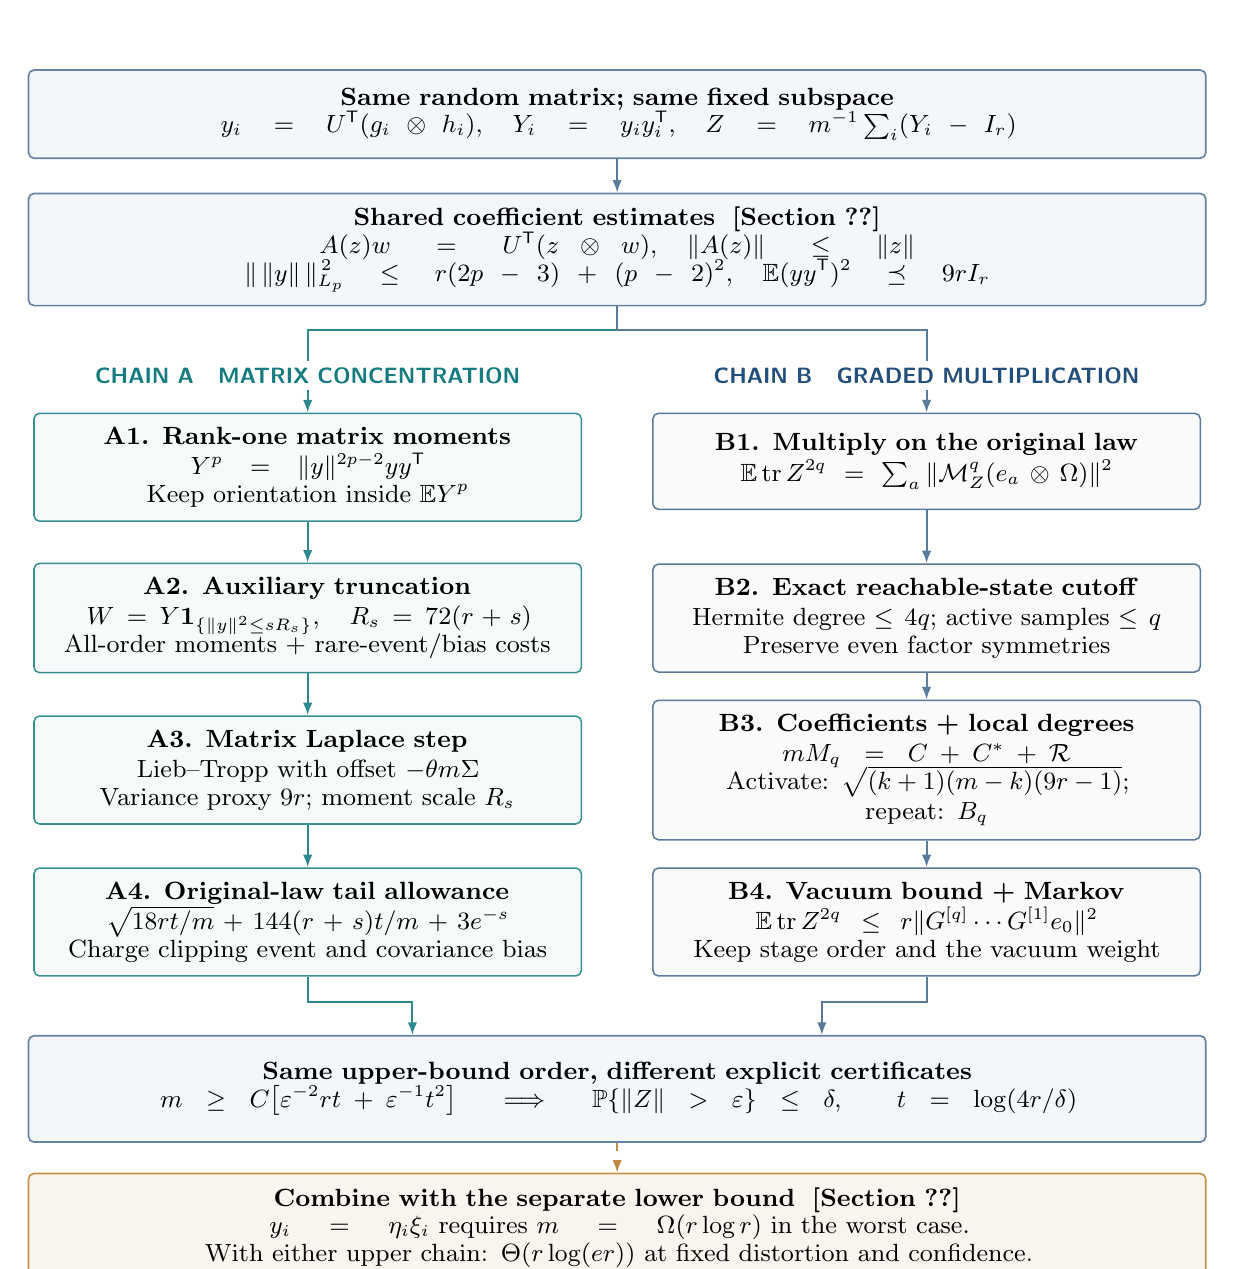
\begin{tikzpicture}[
  x=1cm,y=1cm,>={Latex[length=1.6mm,width=1.2mm]},
  shared/.style={draw=Navy!70,fill=Ice,rounded corners=2pt,
    line width=.6pt,text width=14.6cm,minimum height=1.12cm,
    align=center,inner sep=5pt,font=\small},
  lbox/.style={draw=Amber!80,fill=Amber!8,rounded corners=2pt,
    line width=.6pt,text width=14.6cm,minimum height=1.12cm,
    align=center,inner sep=5pt,font=\small},
  abox/.style={draw=Teal!85,fill=Teal!4,rounded corners=2pt,
    line width=.55pt,text width=6.6cm,minimum height=1.22cm,
    align=center,inner sep=5pt,font=\small},
  bbox/.style={draw=Navy!75,fill=Navy!3,rounded corners=2pt,
    line width=.55pt,text width=6.6cm,minimum height=1.22cm,
    align=center,inner sep=5pt,font=\small},
  flow/.style={->,line width=.7pt,draw=Navy!75},
  aflow/.style={->,line width=.7pt,draw=Teal!90},
  labeltext/.style={font=\sffamily\bfseries\footnotesize,align=center,
    fill=white,inner sep=2.5pt}
]
\node[shared] (model) at (0,0) {\textbf{Same random matrix; same fixed subspace}\\[-1pt]
  $y_i=U^{\mathsf T}(g_i\otimes h_i),\quad Y_i=y_i y_i^{\mathsf T},\quad
  Z=m^{-1}\sum_i(Y_i-I_r)$};
\node[shared,minimum height=1.26cm] (common) at (0,-1.72) {\textbf{Shared coefficient estimates \;[Section~\ref{sec:common}]}\\[-1pt]
  $A(z)w=U^{\mathsf T}(z\otimes w),\quad \|A(z)\|\le\|z\|$\\[-1pt]
  $\|\,\|y\|\,\|_{L_p}^{\,2}\le r(2p-3)+(p-2)^2,\quad
   \mathbb E(yy^{\mathsf T})^2\preceq9rI_r$};
\draw[flow] (model)--(common);
% Row 1 is anchored at a common top edge (A1 is one line taller than B1),
% so the two branch arrows have equal length.
\node[abox,anchor=north] (a1) at (-3.93,-3.79) {\textbf{A1. Rank-one matrix moments}\\
  $Y^p=\|y\|^{2p-2}yy^{\mathsf T}$\\[-1pt]
  Keep orientation inside $\mathbb E Y^p$};
\node[bbox,anchor=north] (b1) at (3.93,-3.79) {\textbf{B1. Multiply on the original law}\\
  $\mathbb E\operatorname{tr} Z^{2q}
    =\sum_a\|\mathcal M_Z^q(e_a\otimes\Omega)\|^2$};
% Branch arrows are drawn first; the white-filled chain labels then sit on top
% of the vertical segments, so no arrowhead touches the label text.
\draw[aflow] (common.south)--++(0,-.30)-|(a1.north);
\draw[flow] (common.south)--++(0,-.30)-|(b1.north);
\node[labeltext,text=Teal] at (-3.93,-3.32) {CHAIN A\quad MATRIX CONCENTRATION};
\node[labeltext,text=Navy] at (3.93,-3.32) {CHAIN B\quad GRADED MULTIPLICATION};
\node[abox] (a2) at (-3.93,-6.40) {\textbf{A2. Auxiliary truncation}\\
  $W=Y\mathbf1_{\{\|y\|^2\le sR_s\}},\quad R_s=72(r+s)$\\[-1pt]
  All-order moments + rare-event/bias costs};
\node[bbox] (b2) at (3.93,-6.40) {\textbf{B2. Exact reachable-state cutoff}\\
  Hermite degree $\le4q$; active samples $\le q$\\[-1pt]
  Preserve even factor symmetries};
\draw[aflow] (a1)--(a2);\draw[flow] (b1)--(b2);
\node[abox] (a3) at (-3.93,-8.33) {\textbf{A3. Matrix Laplace step}\\
  Lieb--Tropp with offset $-\theta m\Sigma$\\[-1pt]
  Variance proxy $9r$; moment scale $R_s$};
\node[bbox] (b3) at (3.93,-8.33) {\textbf{B3. Coefficients + local degrees}\\
  $mM_q=C+C^*+\mathcal R$\\[-1pt]
  Activate: $\sqrt{(k+1)(m-k)(9r-1)}$; repeat: $B_q$};
\draw[aflow] (a2)--(a3);\draw[flow] (b2)--(b3);
\node[abox] (a4) at (-3.93,-10.26) {\textbf{A4. Original-law tail allowance}\\
  $\sqrt{18rt/m}+144(r+s)t/m+3e^{-s}$\\[-1pt]
  Charge clipping event and covariance bias};
\node[bbox] (b4) at (3.93,-10.26) {\textbf{B4. Vacuum bound + Markov}\\
  $\mathbb E\operatorname{tr}Z^{2q}\le
    r\|G^{[q]}\cdots G^{[1]}e_0\|^2$\\[-1pt]
  Keep stage order and the vacuum weight};
\draw[aflow] (a3)--(a4);\draw[flow] (b3)--(b4);
\node[shared,minimum height=1.35cm] (end) at (0,-12.38) {\textbf{Same upper-bound order, different explicit certificates}\\[-1pt]
  $m\ge C\bigl[\varepsilon^{-2}rt+\varepsilon^{-1}t^2\bigr]
   \;\Longrightarrow\;\mathbb P\{\|Z\|>\varepsilon\}\le\delta,
   \qquad t=\log(4r/\delta)$};
% The two chains enter the endpoint box at separate points, so the merge
% arrows neither overlap nor stack their arrowheads.
\draw[aflow] (a4.south)--++(0,-.32)-|([xshift=-2.6cm]end.north);
\draw[flow] (b4.south)--++(0,-.32)-|([xshift=2.6cm]end.north);
\node[lbox] (lower) at (0,-14.14) {\textbf{Combine with the separate lower bound \;[Section~\ref{sec:lower}]}\\[-1pt]
  $y_i=\eta_i\xi_i$ requires $m=\Omega(r\log r)$ in the worst case.\\[-1pt]
  With either upper chain: $\Theta(r\log(er))$ at fixed distortion and confidence.};
\draw[flow,draw=Amber!85,dashed] (end.south)--(lower.north);
\end{tikzpicture}%
}
\end{center}
\vfill
{\footnotesize\color{Ink!75}
All application-specific steps and the matching lower bound are included here.
Standard analytic inputs are stated explicitly and attributed. Numerical entries are
sufficient theorem certificates, not empirical sample sizes. This research derivation
has not been independently externally audited or formally verified.}
\clearpage

\section{Model, theorem, and comparison at a glance}\label{sec:model}
\subsection{The unchanged sketch and its quantifiers}
Let $n_1,n_2,r,m\ge1$ be integers with $r\le n_1n_2$, and fix a deterministic isometry
\[
 U:\R^r\longrightarrow\R^{n_1}\otimes\R^{n_2},\qquad U^{\mathsf T}U=I_r.
\]
For $1\le i\le m$, let $g_i\sim N(0,I_{n_1})$ and $h_i\sim N(0,I_{n_2})$;
all samples and both factors are mutually independent. Define
\begin{equation}\label{eq:model}
 \begin{aligned}
 S&=\frac1{\sqrt m}\begin{pmatrix}(g_1\otimes h_1)^{\mathsf T}\\\vdots\\(g_m\otimes h_m)^{\mathsf T}\end{pmatrix},
 &y_i&=U^{\mathsf T}(g_i\otimes h_i),\\
 Y_i&=y_iy_i^{\mathsf T},\qquad X_i=Y_i-I_r,
 &Z&=U^{\mathsf T}S^{\mathsf T}SU-I_r=\frac1m\sum_{i=1}^mX_i.
 \end{aligned}
\end{equation}
Independence gives $\E(g_i\otimes h_i)(g_i\otimes h_i)^{\mathsf T}=I_{n_1n_2}$,
so $\E Y_i=I_r$ and $\E X_i=0$.
The event $\norm Z\le\varepsilon$ is exactly the squared-norm embedding guarantee
\[
 (1-\varepsilon)\norm x^2\le\norm{SUx}^2\le(1+\varepsilon)\norm x^2
 \quad\text{for every }x\in\R^r.
\]
Every probability statement below is for \emph{each fixed} $U$, with constants uniform
in $U,n_1,n_2$. It is not a simultaneous statement for all subspaces after $S$ is drawn.
All logarithms are natural; unmarked matrix norms are operator norms.

\begin{theorem}[Common endpoint]\label{thm:common-endpoint}
There is a universal $C>0$ such that, for $0<\varepsilon,\delta<1$ and
$t=\log(4r/\delta)$,
\begin{equation}\label{eq:main-size}
 m\ge C\left(\frac{rt}{\varepsilon^2}+\frac{t^2}{\varepsilon}\right)
 \quad\Longrightarrow\quad\Prob\{\norm Z>\varepsilon\}\le\delta.
\end{equation}
Both proof chains below establish this upper bound independently after their shared
local estimates. Conversely, for $Ue_a=e_a\otimes e_1$ with $n_1=r,n_2=2$, there is
$c>0$ such that uniformly over integers $1\le m\le c r\log r$,
\[
 \Prob\{\norm Z>1/2\}\longrightarrow1\qquad(r\longrightarrow\infty).
\]
Therefore the worst-case sample order at distortion $1/2$ and success probability
$0.99$ is $\Theta(r\log(er))$.
\end{theorem}
The statement does not assert optimal joint dependence on $\varepsilon$ and $\delta$.
The upper bound is proved for arbitrary subspace coefficients; only the lower-bound
example uses a common factor.

\subsection{Where the chains differ}
\begingroup\small\setlength{\tabcolsep}{5pt}\renewcommand{\arraystretch}{1.25}
\begin{tabularx}{\textwidth}{@{}P{.21\textwidth}YY@{}}
\toprule
\textbf{Feature}&\textbf{Chain A: matrix concentration}&\textbf{Chain B: graded multiplication}\\
\midrule
Shared starting point&\multicolumn{2}{P{.73\textwidth}}{The exact map $A(z)w=U^{\mathsf T}(z\otimes w)$, projected-row moments, and directional fourth moments.}\\
Object retained&One-row matrix powers $\E Y^p$.&The full original-law vacuum walk and its sample/degree sectors.\\
Cutoff&Auxiliary rare-outcome truncation $\norm y^2\le sR_s$; probability and bias are paid.&Exact Hermite reachability and active-sample cutoff; no outcome is removed.\\
Main assembly tool&Lieb's trace concavity, iterated as the matrix Laplace method.&Fresh-sample and repeated-visit contractions, followed by nonnegative vacuum propagation.\\
Explicit output&Tail allowance in \eqref{eq:A-tail}.&Untruncated moments; stationary, stage-dependent, and closed-form certificates.\\
Constants&One specified conservative baseline.&Closed form can be worse; stage-dependent certificates improve this baseline in the reported cases.\\
Additional consequence&Not claimed from its truncated certificate.&Exact $2q$-wise sample-block moment transfer.\\
\bottomrule
\end{tabularx}
\endgroup

\subsection{How to read this note}
Section~\ref{sec:common} proves the shared coefficient estimates.
Sections~\ref{sec:A} and~\ref{sec:B} are the two upper-bound chains.
Section~\ref{sec:lower} supplies the common lower bound;
Section~\ref{sec:comparison} compares fully specified constants and numerical certificates.
Appendices give the Gaussian normalization, the constant-$72$ verification,
and the numerical recurrence. No earlier project manuscript is needed to check an
application-specific step.

Gaussian hypercontractivity is credited to Nelson, and the logarithmic Sobolev
inequality and its semigroup connection to Gross~\cite{Nelson,Gross,GrossSurvey}; short derivations are included in
Appendix~\ref{app:gaussian}. Chain A also uses Lieb's trace-concavity theorem, stated
explicitly in Section~\ref{sec:A-laplace}; that classical theorem is the one analytic
input not reproved here. The matrix concentration step is derived from it, rather
than quoted as a black box. Chain B does not use it.

\clearpage
\subsection{Related work and attribution}\label{sec:attribution-intro}
The sketch is not a new construction. Tensor random projections were studied by
Sun, Guo, Tropp, and Udell~\cite{Sun}, and fixed-vector polynomial-kernel sketching
bounds appear in Ahle et al.~\cite[Appendix~A.2, Theorem~42]{Ahle}.
In particular, the order of the $r=1$ sample bound is already present in that
fixed-vector literature; the target
here is uniformity over all directions of an arbitrary fixed $r$-dimensional
subspace. Bujanovi\'c and Kressner~\cite{BK} study norm and trace estimation with
random rank-one vectors. Bujanovi\'c, Grubi\v{s}i\'c, Kressner, and
Lam~\cite{BGKL} prove an earlier OSE theorem for this two-factor Gaussian model.

Beretta--Musco~\cite[Theorem~1.3]{BM} give
$O(\varepsilon^{-2}r\log^3(r/(\varepsilon\delta)))$ rows in the Gaussian
order-two specialization. Their theorem covers more distributions and tensor
orders. The comparison here is restricted to that specialization, with an
absolute rescaling of distortion when passing between norm and squared-norm
conventions. Neither the present constants nor the numerical table are advertised
as universal improvements over their broader result.

\paragraph{A version-sensitive predecessor.}
Saibaba, Verma, and Ballard's first version~\cite[Theorem~11]{SVBv1}
contains a near-linear, polylogarithmic OSE claim and an accompanying proof
attempt. The second version~\cite{SVBv2} omits that assertion. Beretta--Musco's
acknowledgments~\cite{BM} report that a proof error prompted its removal and
credit the earlier strategy. We retain this historical credit but do not use the
removed assertion as a theorem. The paper as a whole is not described as withdrawn.

\paragraph{Methodological antecedents.}
Chain A follows the established truncation-and-concentration architecture for
Khatri--Rao sketches; compare~\cite[Section~2.3]{BM}. Its specific calculations
retain one-row matrix moments and the distinction between the truncation height
and the exponential-moment scale. The matrix Laplace mechanism is the
Lieb--Tropp method, not a new concentration theorem~\cite{Lieb,Tropp}.
The order of the shared projected-row estimate also follows from the Hilbert-space
specialization of Adamczak--Lata\l a--Meller~\cite[Corollary~12]{ALM};
Section~\ref{sec:common} supplies an explicit normalization and a short direct proof.
Coefficient-sensitive matrix-chaos estimates and Khatri--Rao applications also
precede this note in Bandeira, Lucca, Nizi\'c-Nikolac, and
van Handel~\cite{BLNvH}. Their full-matrix norm estimates are not identified with
the centered, arbitrary-fixed-subspace covariance theorem proved here.

Chain B is organized using the supplied framework~\cite{Framework}. Its
multiplication representation, Hermite decomposition, and Jacobi moment
interpretation have classical antecedents~\cite{Wiener,AccardiBozejko,GolubWelsch}.
The application-specific content to assess is the sequence of local estimates,
the resulting sample bound, and its explicit vacuum certificates, rather than
ownership of these representation principles. Section~\ref{sec:provenance-table}
separates the sources and roles. No publication-priority claim is made.

\clearpage
\section{Shared coefficient estimates}\label{sec:common}
\begin{takeaway}
The same subspace geometry feeds both chains. Keep the map $A(z)$ collected before
taking norms: its operator-norm Lipschitz constant is $1$, not $\sqrt r$.
Then keep the rank-one orientation when a matrix-valued estimate is needed.
\end{takeaway}

\subsection{Gaussian moment control with explicit normalization}
Write $\gamma_N$ for standard Gaussian measure on $\R^N$ and
$\Ent(F)=\E[F\log F]-(\E F)\log\E F$ for $F\ge0$.
The Gaussian logarithmic Sobolev inequality is
\begin{equation}\label{eq:LSI}
 \Ent_{\gamma_N}(f^2)\le2\E_{\gamma_N}\norm{\nabla f}^2.
\end{equation}
For a Hilbert-valued homogeneous Hermite polynomial $F_d$ of total degree $d$,
Gaussian hypercontractivity gives
\begin{equation}\label{eq:HC}
 \norm{F_d}_{L_u}\le(u-1)^{d/2}\norm{F_d}_{L_2},\qquad u\ge2.
\end{equation}
The normalization and short semigroup proofs appear in Appendix~\ref{app:gaussian};
these are classical Nelson--Gross inequalities~\cite{Nelson,Gross,GrossSurvey}.
Differentiating moments under a logarithmic Sobolev inequality is also a standard
route to moment estimates; see Aida--Stroock~\cite{AidaStroock}.
The following lemma fixes the Gaussian normalization used throughout.

\begin{lemma}[Lipschitz moments]\label{lem:lip}
For a nonnegative $L$-Lipschitz function $f$ on a finite-dimensional standard
Gaussian space and any real $p\ge2$,
\begin{equation}\label{eq:lip}
 \norm f_{L_p}^2\le\norm f_{L_2}^2+(p-2)L^2.
\end{equation}
\end{lemma}
\begin{proof}
Assume first that $f$ is smooth, bounded, and bounded below by a positive
constant, and set $M(p)=\E f^p$.

\step{1. Differentiate the running moment in its exponent.}
Since $\frac{d}{dp}\E f^p=\E f^p\log f$, a direct computation gives
\[
 \frac{d}{dp}M(p)^{2/p}
 =\frac2{p^2}M(p)^{2/p-1}\Ent(f^p).
\]

\step{2. Bound the entropy by the logarithmic Sobolev inequality.}
Apply \eqref{eq:LSI} to $f^{p/2}$ and use $\norm{\nabla f}\le L$:
\[
 \Ent(f^p)\le\frac{p^2L^2}2\,\E f^{p-2}.
\]
H\"older's inequality gives $\E f^{p-2}\le M(p)^{(p-2)/p}$, so the two previous
displays combine into
\[
 \frac{d}{dp}M(p)^{2/p}
 \le L^2M(p)^{2/p-1}M(p)^{1-2/p}=L^2.
\]

\step{3. Integrate from $2$ to $p$.}
This yields $M(p)^{2/p}\le M(2)+(p-2)L^2$, which is \eqref{eq:lip}.
Smoothing, a positive regularization, and truncation of the scalar test function
justify the same bound for Lipschitz $f$ by passage to the limit.
\end{proof}

\subsection{The collective conditional Gaussian map}
Reshape the columns of $U$ as matrices $B_1,\ldots,B_r\in\R^{n_1\times n_2}$.
Then
\begin{equation}\label{eq:B-orthonormal}
 \tr(B_a^{\mathsf T}B_b)=\delta_{ab},\qquad
 y_a=g^{\mathsf T}B_a h.
\end{equation}
For $z\in\R^{n_1}$ define $A(z):\R^{n_2}\to\R^r$ by
\begin{equation}\label{eq:A-map}
 A(z)w=U^{\mathsf T}(z\otimes w),\qquad y=A(g)h.
\end{equation}
Because $U^{\mathsf T}$ is a contraction,
\begin{equation}\label{eq:collective}
 \norm{A(z)}\le\norm z,\qquad
 \E\norm{A(g)}_\F^2=r,\qquad
 \norm{A(z)}_\F^2\le r\norm z^2.
\end{equation}
The second assertion follows by summing $\norm{B_a}_\F^2=1$; the third follows from
$\sum_a\norm{B_a^{\mathsf T}z}^2\le\sum_a\norm{B_a}_\F^2\norm z^2$.
Linearity of $A$ makes $z\mapsto\norm{A(z)}$ $1$-Lipschitz and
$z\mapsto\norm{A(z)}_\F$ $\sqrt r$-Lipschitz.

\begin{lemma}[Projected-row moments]\label{lem:row}
For every real $p\ge2$,
\begin{equation}\label{eq:row}
 \boxed{\bigl\|\norm y\bigr\|_{L_p}^{\,2}
 \le r(2p-3)+(p-2)^2.}
\end{equation}
In particular $\|\norm y\|_{L_p}\le\sqrt{2rp}+p$.
\end{lemma}
\begin{proof}
\step{1. Bound the moments of the two Lipschitz norms of $A(g)$.}
By \eqref{eq:collective}, $z\mapsto\norm{A(z)}_\F$ is $\sqrt r$-Lipschitz with
squared $L_2$ norm $r$, and $z\mapsto\norm{A(z)}$ is $1$-Lipschitz with squared
$L_2$ norm at most $r$. Lemma~\ref{lem:lip} gives
\[
 \bigl\|\norm{A(g)}_\F\bigr\|_{L_p}^2\le r(p-1),\qquad
 \bigl\|\norm{A(g)}\bigr\|_{L_p}^2\le r+p-2.
\]

\step{2. Condition on $g$ and integrate over $h$.}
For fixed $g$, the function $h\mapsto\norm{A(g)h}$ has Lipschitz constant
$\norm{A(g)}$ and squared $L_2$ norm $\norm{A(g)}_\F^2$. Lemma~\ref{lem:lip},
applied in the variable $h$ alone, gives
\[
 (\E_h\norm{A(g)h}^p)^{2/p}
 \le\norm{A(g)}_\F^2+(p-2)\norm{A(g)}^2.
\]

\step{3. Combine the two factor bounds.}
Take $L_{p/2}$ norms in $g$ on both sides. Minkowski's inequality in $L_{p/2}$
separates the two summands on the right, and Step~1 bounds each of them:
\[
 \bigl\|\norm y\bigr\|_{L_p}^2
 \le r(p-1)+(p-2)(r+p-2)
 =r(2p-3)+(p-2)^2.
\]
All coefficients remain collected. No common Schmidt basis and no independence of
the coordinates of $y$ is assumed.
\end{proof}

\paragraph{Relation to Banach-space Gaussian chaos bounds.}
The order $\|\norm y\|_{L_p}\lesssim\sqrt{rp}+p$ is already a consequence of
Adamczak--Lata\l a--Meller~\cite[Corollary~12]{ALM}, with their function-space
exponent set to $2$. To check the specialization, set
$c_{ij}=U^{\mathsf T}(e_i\otimes e_j)$ and encode the bilinear form using the
symmetric coefficient array with cross blocks $c_{ij}/2$ and zero diagonal
blocks, acting on the concatenated Gaussian $(g,h)$. The four coefficient
quantities in that corollary are bounded, in their displayed order, by
$\sqrt{r/2}$, $\sqrt r/2$, $1/\sqrt2$, and $1/2$.
This gives the stated order. Lemma~\ref{lem:row} supplies the explicit bound
\eqref{eq:row}, not a claim that this moment order is new. The cited corollary
is an antecedent for the shared local estimate, not by itself the centered
sample-covariance theorem.

\subsection{Directional fourth moments and matrix variance}
The normal fourth-moment calculation below is a special case of Isserlis's
product-moment formula~\cite{Isserlis}, written out to fix the constant $9$.
For the related rank-one probing model, see also~\cite{BK}.
\begin{lemma}[Fourth moments]\label{lem:four}
For every $x\in\R^r$,
\begin{equation}\label{eq:four}
 \E\ip{x}{y}^4\le9\norm x^4.
\end{equation}
Consequently, with $Y=yy^{\mathsf T}$ and $X=Y-I_r$,
\begin{equation}\label{eq:variance}
 \E Y^2\preceq9rI_r,\qquad
 \E X^2\preceq v_r I_r,\qquad v_r:=9r-1.
\end{equation}
\end{lemma}
\begin{proof}
\step{1. The directional fourth moment.}
For unit $x$, put $B_x=\sum_a x_aB_a$. Equation~\eqref{eq:B-orthonormal} gives
$\norm{B_x}_\F=1$. Conditional on $g$, $g^{\mathsf T}B_xh$ is Gaussian with
variance $g^{\mathsf T}Qg$, where $Q=B_xB_x^{\mathsf T}\succeq0$ and $\tr Q=1$.
Diagonalizing $Q$ gives
\[
 \E\ip{x}{y}^4=3\E(g^{\mathsf T}Qg)^2
 =3(\tr Q)^2+6\tr Q^2\le9.
\]
Homogeneity proves \eqref{eq:four}.

\step{2. The matrix second moment.}
For unit $x$, Cauchy--Schwarz in each summand gives
\[
 x^{\mathsf T}(\E Y^2)x
 =\sum_{a=1}^r\E[y_a^2\ip{x}{y}^2]
 \le\sum_{a=1}^r(\E y_a^4)^{1/2}(\E\ip{x}{y}^4)^{1/2}
 \le9r.
\]

\step{3. Center.}
Finally $\E X^2=\E Y^2-2\E Y+I_r=\E Y^2-I_r$.
\end{proof}
The common-factor case $y=\eta\xi$ has
$\|\norm y\|_{L_p}=\|\eta\|_{L_p}\|\norm\xi\|_{L_p}$, of order
$\sqrt{rp}+p$. It calibrates the uniform order of Lemma~\ref{lem:row}, but is not
used to restrict its upper-bound hypotheses.

\clearpage
\section{Chain A: matrix moments, truncation, and concentration}\label{sec:A}
\begin{takeaway}
Chain A never constructs a graded multiplication operator. It converts the common
row estimates into operator-valued moments of one rank-one matrix, truncates only
for the exponential series, and uses matrix Laplace concentration. The final
statement is for the original, unmodified sketch.
\end{takeaway}

The overall architecture has direct precedents in the Khatri--Rao literature
identified in Section~\ref{sec:attribution-intro}. Reproving the concentration
step below does not make that step, or the use of a truncated sample covariance,
a new general method. The displayed constants belong to the implementation in
this note.

\subsection{A1. Keep matrix orientation when estimating powers}
\begin{lemma}[Explicit one-row matrix moments]\label{lem:raw-moments}
For $Y=yy^{\mathsf T}$ and every integer $p\ge3$,
\begin{align}
 \E Y^p
 &\preceq 3\bigl[(8p-11)r+(4p-6)^2\bigr]^{p-1}I_r,\label{eq:raw-moment}\\
 \E Y^p
 &\preceq\frac{p!}{2}\,9r\,[72(r+p)]^{p-2}I_r.\label{eq:72-moment}
\end{align}
For $p=2$, $\E Y^2\preceq9rI_r$.
\end{lemma}
\begin{proof}
\step{1. Bound each directional moment of the matrix power.}
The rank-one identity
\[
 Y^p=\norm y^{2p-2}yy^{\mathsf T}
\]
lets us keep the direction $x$ until after expectation. For any unit $x$,
\begin{align*}
 x^{\mathsf T}(\E Y^p)x
 &=\E\bigl[\norm y^{2p-2}\ip{x}{y}^2\bigr]\\
 &\le(\E\norm y^{4p-4})^{1/2}(\E\ip{x}{y}^4)^{1/2}\\
 &\le3\bigl\|\norm y\bigr\|_{L_{4p-4}}^{2p-2}\\
 &\le3\bigl[(8p-11)r+(4p-6)^2\bigr]^{p-1}.
\end{align*}
The second line is Cauchy--Schwarz; the third bounds the directional factor by
Lemma~\ref{lem:four}; the last applies Lemma~\ref{lem:row} at exponent $4p-4$.
Since $x$ is arbitrary, this proves \eqref{eq:raw-moment} as a Loewner bound.

\step{2. Pass to the uniform moment scale $72(r+p)$.}
The scalar inequality
\begin{equation}\label{eq:72-scalar}
 3\bigl[(8p-11)r+(4p-6)^2\bigr]^{p-1}
 \le\frac{p!}{2}\,9r\,[72(r+p)]^{p-2}
\end{equation}
is proved for every $r\ge1,p\ge3$ in Appendix~\ref{app:72}, giving
\eqref{eq:72-moment}. The $p=2$ case is Lemma~\ref{lem:four}.
\end{proof}
The distinction is between $\norm{\E Y^p}$ and $\E\norm{Y}^p$.
Replacing $Y$ by its norm before taking expectation discards the direction used above.

\subsection{A2. Truncate without paying the full cutoff height}
The untruncated $Y$ need not have a finite positive exponential moment. For example,
when $r=1$ and $y=gh$, $Y=g^2h^2$ has infinite moment-generating function at every
positive argument. Conditional on $g$, the Gaussian integral in $h$ already diverges
whenever $2\theta g^2\ge1$, an event of positive probability.
Thus a positive-matrix exponential theorem cannot be applied to $Y$ directly.

\begin{lemma}[All-order moments of a bounded auxiliary matrix]\label{lem:truncate}
Fix an integer $s\ge2$ and define
\begin{equation}\label{eq:truncation}
 R_s=72(r+s),\qquad L_s=sR_s,\qquad
 W=Y\one_{\{\norm y^2\le L_s\}},\qquad\Sigma=\E W.
\end{equation}
Then
\begin{align}
 \Prob\{W\ne Y\}&\le e^{-2s},\label{eq:clip}\\
 0\preceq I_r-\Sigma&\preceq3e^{-s}I_r,\label{eq:bias}\\
 \E W^p&\preceq\frac{p!}{2}\,9r\,R_s^{p-2}I_r
 \qquad\text{for every integer }p\ge2.\label{eq:all-order}
\end{align}
\end{lemma}
\begin{proof}
\step{1. Bound the event on which the sample is changed.}
At exponent $2s$, Lemma~\ref{lem:row} gives
\[
 \bigl\|\norm y^2\bigr\|_{L_s}
 \le r(4s-3)+(2s-2)^2\le4s(r+s).
\]
Markov's inequality therefore gives
\[
 \Prob\{\norm y^2>L_s\}
 \le\left(\frac{4s(r+s)}{72s(r+s)}\right)^s
 =18^{-s}\le e^{-2s}.
\]

\step{2. Charge the covariance bias in each direction.}
For a unit vector $x$, Lemma~\ref{lem:four} and Cauchy--Schwarz imply
\[
 x^{\mathsf T}(I_r-\Sigma)x
 =\E\bigl[\ip{x}{y}^2\one_{\{\norm y^2>L_s\}}\bigr]
 \le3\Prob\{\norm y^2>L_s\}^{1/2}\le3e^{-s}.
\]
The integrand is nonnegative, proving both sides of \eqref{eq:bias}.

\step{3. Prove the matrix moment bound through order $s$.}
For $p=2$, $\E W^2\preceq\E Y^2\preceq9rI_r$.
For $3\le p\le s$, the scalar event in \eqref{eq:truncation} gives
$W^p\preceq Y^p$ pointwise. Lemma~\ref{lem:raw-moments} and $p\le s$ yield
\[
 \E W^p\preceq\frac{p!}{2}\,9r\,[72(r+p)]^{p-2}I_r
 \preceq\frac{p!}{2}\,9r\,R_s^{p-2}I_r.
\]

\step{4. Extend to every order required by the exponential series.}
For an integer $p>s$, spectral calculus on $0\preceq W\preceq L_sI_r$ gives
\[
 W^p\preceq L_s^{p-s}W^s.
\]
Consequently,
\[
 \E W^p\preceq\frac{s!}{2}\,9r\,R_s^{s-2}L_s^{p-s}I_r
 =\frac{s!s^{p-s}}{2}\,9r\,R_s^{p-2}I_r
 \preceq\frac{p!}{2}\,9r\,R_s^{p-2}I_r.
\]
The last inequality follows by comparing each factor of
$(s+1)(s+2)\cdots p$ with $s$. This proves all of \eqref{eq:all-order},
not just the first $s$ moments.
\end{proof}
\begin{takeaway}
The almost-sure cutoff height is $L_s=sR_s$, but the matrix moment-growth scale is
only $R_s$. Charging $L_s$ as the bounded-summand scale would lose the factor $s$.
\end{takeaway}

\subsection{A3. A matrix Laplace step with valid centering}\label{sec:A-laplace}
The classical matrix-analysis input is Lieb's trace-concavity theorem: for a fixed
self-adjoint $H$, the map
\begin{equation}\label{eq:lieb}
 Q\longmapsto\tr\exp(H+\log Q)
\end{equation}
is concave on the positive-definite cone~\cite{Lieb,Tropp}.
We use no assumption that a random matrix commutes with its expectation.

\begin{lemma}[Matrix Laplace iteration with an offset]\label{lem:laplace}
For independent self-adjoint random matrices $A_1,\ldots,A_m$ with finite matrix
exponential moments, and deterministic self-adjoint $H$,
\begin{equation}\label{eq:laplace}
 \E\tr\exp\left(H+\sum_{i=1}^mA_i\right)
 \le\tr\exp\left(H+\sum_{i=1}^m\log\E e^{A_i}\right).
\end{equation}
\end{lemma}
\begin{proof}
For one random matrix $A$, write $Q=e^A$. Jensen's inequality applied to
\eqref{eq:lieb} gives
\[
 \E\tr\exp(H+A)\le\tr\exp(H+\log\E e^A).
\]
For the sum, condition first on $A_1,\ldots,A_{m-1}$, treating all their terms as
part of $H$. Independence makes $\log\E e^{A_m}$ deterministic. Repeat for
$A_{m-1},\ldots,A_1$. This is the matrix Laplace iteration used by Tropp;
no reordering of products or commuting-mean identity is involved~\cite{Tropp}.
\end{proof}

The next lemma is the positive-raw-moment version of the usual subexponential
matrix Bernstein argument~\cite[Theorem~6.2 and Lemma~6.8]{Tropp}.
Its proof uses the deterministic offset in Lemma~\ref{lem:laplace} so that no
commutation of a sample and its mean is assumed; it is not presented as a new
abstract concentration inequality.

\begin{lemma}[Concentration from positive matrix moments]\label{lem:bernstein}
Let $W_1,\ldots,W_m$ be independent, identically distributed bounded positive
semidefinite $r\times r$ matrices with $\E W_i=\Sigma$. Suppose that for $p\ge2$,
\[
 \E W_i^p\preceq\frac{p!}{2}\,vR^{p-2}I_r.
\]
Then for every $u>0$,
\begin{equation}\label{eq:bernstein}
 \Prob\left\{\left\|\frac1m\sum_iW_i-\Sigma\right\|
 >\sqrt{\frac{2vu}{m}}+\frac{2Ru}{m}\right\}\le2re^{-u}.
\end{equation}
\end{lemma}
\begin{proof}
\step{1. Bound the logarithm of the uncentered exponential moment.}
For $|\theta|R<1$, positivity of each $W_i^p$ and the exponential series imply
\[
 \E e^{\theta W_i}-I_r-\theta\Sigma
 \preceq\sum_{p\ge2}\frac{|\theta|^p}{p!}\E W_i^p
 \preceq\frac{\theta^2v}{2(1-|\theta|R)}I_r.
\]
For positive definite $Q$, spectral calculus gives $\log Q\preceq Q-I_r$.
Therefore
\begin{equation}\label{eq:log-mgf}
 \log\E e^{\theta W_i}
 \preceq\theta\Sigma+
 \frac{\theta^2v}{2(1-|\theta|R)}I_r.
\end{equation}

\step{2. Center by a deterministic offset inside the trace exponential.}
In Lemma~\ref{lem:laplace}, take $A_i=\theta W_i$ and $H=-\theta m\Sigma$.
Using \eqref{eq:log-mgf},
\[
 \E\tr\exp\left(\theta\sum_i(W_i-\Sigma)\right)
 \le r\exp\left(\frac{m\theta^2v}{2(1-|\theta|R)}\right).
\]
Here a Loewner bound on the exponent gives a bound on each eigenvalue and hence
on the trace exponential. No operator monotonicity of the exponential is needed.

\step{3. Convert the exponential bound to the two spectral tails.}
For a self-adjoint $D$ and $\theta>0$, the event $\lambda_{\max}(D)>x$ implies
$\tr e^{\theta D}>e^{\theta x}$. Markov, followed by
$\theta=x/(mv+Rx)$, gives
\[
 \Prob\left\{\lambda_{\max}\left(\sum_i(W_i-\Sigma)\right)>x\right\}
 \le r\exp\left(-\frac{x^2}{2(mv+Rx)}\right).
\]
Use negative $\theta$ for the lower spectral tail and add the probabilities.
Finally $x=\sqrt{2mvu}+2Ru$ satisfies $x^2\ge2u(mv+Rx)$, proving
\eqref{eq:bernstein}.
\end{proof}

\subsection{A4. Restore the original samples and solve for \texorpdfstring{$m$}{m}}
\begin{theorem}[Explicit Chain A certificate]\label{thm:A}
Let $t=\log(4r/\delta)$ and $s=\lceil\log(4m/\delta)\rceil$. Then
\begin{equation}\label{eq:A-tail}
 \boxed{\Prob\left\{\norm Z>
 \sqrt{\frac{18rt}{m}}+\frac{144(r+s)t}{m}+3e^{-s}\right\}\le\delta.}
\end{equation}
In particular, having the displayed allowance at most $\varepsilon$ is an explicit
sufficient condition for the embedding guarantee.
\end{theorem}
\begin{proof}
The integer $s$ is at least $2$.

\step{1. Replace every sample by its truncation.}
Apply Lemma~\ref{lem:truncate} separately to the
independent samples, with the same deterministic cutoff. A union bound gives
\[
 \Prob\{\exists i:W_i\ne Y_i\}\le me^{-2s}
 \le\frac{\delta^2}{16m}\le\frac\delta{16}.
\]

\step{2. Concentrate the truncated average.}
Lemma~\ref{lem:bernstein}, with $v=9r$, $R=R_s=72(r+s)$, and $u=t$, fails with
probability at most $2re^{-t}=\delta/2$.

\step{3. Return to the original sketch.}
On the intersection of the two good events, every $W_i$ equals $Y_i$, so
\begin{align*}
 \norm Z
 &\le\left\|\frac1m\sum_iW_i-\Sigma\right\|+\norm{\Sigma-I_r}\\
 &\le\sqrt{\frac{18rt}{m}}+\frac{144(r+s)t}{m}+3e^{-s}.
\end{align*}
The total failure probability is less than $\delta$. The conclusion concerns the
original $S$, not an estimator that clips its rows during execution.
\end{proof}

\begin{proposition}[The common sample order follows from Chain A]\label{prop:A-size}
The explicit certificate \eqref{eq:A-tail} implies \eqref{eq:main-size} with a
universal constant.
\end{proposition}
\begin{proof}
\step{1. Simplify the allowance to two monotone terms.}
Since $s\le\log(4m/\delta)+1$ and $3e^{-s}\le3\delta/(4m)$, the allowance in
\eqref{eq:A-tail} is at most
\begin{equation}\label{eq:A-rough}
 C_1\left[\sqrt{\frac{rt}{m}}+
 \frac{(r+\log(4m/\delta)+1)t}{m}\right]
\end{equation}
for an absolute $C_1$. Both terms decrease with real $m\ge1$; for the second,
differentiate $(r+\log(4m/\delta)+1)/m$.

\step{2. Evaluate at the candidate sample size.}
Set
\[
 m_0=K\left(\frac{rt}{\varepsilon^2}+\frac{t^2}{\varepsilon}\right)
 =K\varepsilon^{-2}t(r+\varepsilon t),\qquad K\ge1.
\]
Here $t>1$, $r\le e^t$, and $t\le e^t$, so
\[
 \log(4m_0/\delta)+1
 \le\log K+2\log(1/\varepsilon)+3t+\log2+1.
\]

\step{3. Bound each term and fix the constant.}
First,
\[
 \sqrt{\frac{rt}{m_0}}\le\frac\varepsilon{\sqrt K}.
\]
Second,
\begin{align*}
 \frac{(r+\log(4m_0/\delta)+1)t}{m_0}
 &\le\frac{\varepsilon^2}{K}
 \frac{r+3t+2\log(1/\varepsilon)+\log K+\log2+1}{r+\varepsilon t}\\
 &\le\frac{C_2(1+\log K)}K\,\varepsilon.
\end{align*}
For the last step, use $r\ge1$, $r+\varepsilon t\ge\varepsilon t$, and
$\varepsilon\log(1/\varepsilon)\le1/e$.
Choose $K$ so that $C_1[K^{-1/2}+C_2(1+\log K)/K]\le1$.
Monotonicity of \eqref{eq:A-rough} handles every larger integer $m$.
\end{proof}

\clearpage
\section{Chain B: exact graded multiplication and vacuum propagation}\label{sec:B}
\begin{takeaway}
Chain B uses the four core stages of the framework: exact multiplication,
reachable graded states, coefficient-sensitive contractions, and vacuum-moment
propagation. No row is clipped and no matrix Laplace theorem is invoked.
The central estimate charges each already-active sample its own local degree
\emph{before} summing over samples.
\end{takeaway}

\subsection{B1. The original-law multiplication identity}
Multiplication in $L_2$ and orthogonal-polynomial coordinates are classical;
Wiener~\cite{Wiener} is a source for homogeneous Gaussian chaos, and
Accardi--Bo\.{z}ejko~\cite{AccardiBozejko} provide a probability-law/creation-operator
representation precedent. We use these as background attributions, not as claims
that either source proves the present embedding theorem. The identity below is
simply Parseval applied to multiplication.
Let
\[
 \mathcal H=\R^r\otimes\bigotimes_{i=1}^m
 L_2(\gamma_{n_1}\otimes\gamma_{n_2}),\qquad \Omega=1.
\]
The external factor $\R^r$ carries the matrix indices, one $L_2$ factor carries
the randomness of one sample, and the vacuum $\Omega$ is the constant function
$1$ in every sample register.
Define $\mathcal M_Zf=Zf$ on the vector polynomials in this Hilbert space.
For an external standard basis vector $e_a$,
\[
 \mathcal M_Z^j(e_a\otimes\Omega)(g_1,h_1,\ldots,g_m,h_m)=Z^je_a.
\]
All of these polynomials are square integrable. The pointwise matrix $Z$ is
symmetric because each $Y_i=y_i y_i^{\mathsf T}$ is symmetric. Thus
$\mathcal M_Z$ is symmetric on its invariant polynomial domain; we do not
assert self-adjointness of this unbounded restriction. The identity follows
directly from $e_a^{\mathsf T}Z^{2q}e_a=\norm{Z^qe_a}^2$ pointwise:
\[
 \E\,e_a^{\mathsf T}Z^{2q}e_a
 =\ip{e_a\otimes\Omega}{\mathcal M_Z^{2q}(e_a\otimes\Omega)}_{\mathcal H}
 =\norm{\mathcal M_Z^q(e_a\otimes\Omega)}_{\mathcal H}^2.
\]
Summing over $a$ gives the identity the chain rests on:
\begin{equation}\label{eq:vacuum}
 \boxed{\E\tr Z^{2q}
 =\sum_{a=1}^r\norm{\mathcal M_Z^q(e_a\otimes\Omega)}_{\mathcal H}^2.}
\end{equation}
The factor $r$ that will eventually arise counts external vacuum seeds. We do not
take a trace over the generally much larger Hermite occupation space.
Every visit to sample $i$ still uses the same $g_i,h_i$.

\subsection{B2. Hermite degree, active samples, and the exact cutoff}
Let $h_\ell=\operatorname{He}_\ell/\sqrt{\ell!}$ denote the normalized probabilists'
Hermite polynomial. Its recurrence is
\begin{equation}\label{eq:Hermite}
 xh_\ell(x)=\sqrt{\ell+1}\,h_{\ell+1}(x)+\sqrt\ell\,h_{\ell-1}(x),
 \qquad h_{-1}=0.
\end{equation}
Products of these functions form an orthonormal basis in each Gaussian sample
space. Let $N_i$ record the total local degree in $(g_i,h_i)$.
Let $P_i$ be the orthogonal projection onto the local constant function, tensored
with identities on all other factors, and put $Q_i=I-P_i$.

\begin{definition}[An active sample]
A sample is active in a product Hermite component when its local factor is
nonconstant, equivalently when it lies in $Q_iL_2$. The exact active set is the
set of such indices. Its size is a second grading, distinct from total degree.
\end{definition}
An active set is not a history of labels that have ever occurred. A sample can
return to its local vacuum, and then be activated again by a later multiplication.

There are exact sign-flip symmetries. Replacing the entire vector $g_i$ by $-g_i$
changes $y_i$ to $-y_i$ but leaves $Y_i$, $X_i$, and $Z$ unchanged; the same holds
for $h_i$. We restrict to functions having even total Hermite degree separately
in every $g_i$ and every $h_i$ register. The vacuum belongs to this subspace,
and multiplication by $Z$ preserves it.

After $j$ multiplications from vacuum,
\begin{equation}\label{eq:reachability}
 \sum_iN_i\le4j,\qquad \#\{\text{active samples}\}\le j.
\end{equation}
Indeed, $X_i$ has polynomial degree at most four and acts on only one sample.

Let $\Pi_q$ project onto the symmetry subspace with total degree at most $4q$
and at most $q$ active samples, and set
\begin{equation}\label{eq:cutoff}
 M_q=\Pi_q\mathcal M_Z\Pi_q.
\end{equation}
This finite-dimensional compression is symmetric, hence self-adjoint.
Inducting on $j$ using
\eqref{eq:reachability} gives
\begin{equation}\label{eq:exact-cutoff}
 M_q^j(e_a\otimes\Omega)=\mathcal M_Z^j(e_a\otimes\Omega),\qquad 0\le j\le q.
\end{equation}
Thus \eqref{eq:vacuum} remains exact with $M_q$ in place of $\mathcal M_Z$.
This is the elementary finite-moment compression principle as organized in the
framework~\cite{Framework}; its proof here is the reachability induction just
given. Neither that induction nor the underlying polynomial representation is
claimed as a new general theorem. No bound on the full unbounded Gaussian
multiplication operator is required.

\subsection{B3. Split activation, return, and repeated visits}
Write $\mathcal X_i$ for multiplication by $X_i$. Centering is the exact identity
$P_i\mathcal X_iP_i=0$. Therefore
\[
 \mathcal X_i=Q_i\mathcal X_iP_i+P_i\mathcal X_iQ_i+Q_i\mathcal X_iQ_i.
\]
Define, on the common cutoff,
\begin{equation}\label{eq:C-R}
 C=\Pi_q\sum_iQ_i\mathcal X_iP_i\Pi_q,\qquad
 \mathcal R=\Pi_q\sum_iQ_i\mathcal X_iQ_i\Pi_q.
\end{equation}
Then
\begin{equation}\label{eq:decomposition}
 \boxed{M_q=\frac1m(C+C^*+\mathcal R).}
\end{equation}
The operator $C$ increases active-sample count by one; $C^*$ decreases it by one;
$\mathcal R$ preserves the exact active set. These are actual full-space
compressions, so using adjointness is legitimate.
Let $\mathcal K_k$ denote the cutoff sector with exactly $k$ active samples.

\subsubsection{Activation and return are controlled by matrix variance}
\begin{lemma}[Fresh-sample contraction]\label{lem:fresh}
With $v_r=9r-1$, for $0\le k<\min(q,m)$,
\begin{equation}\label{eq:fresh}
 \norm{C:\mathcal K_k\to\mathcal K_{k+1}}
 \le\sqrt{(k+1)(m-k)v_r}.
\end{equation}
The reverse map $C^*$ has the same bound.
\end{lemma}
\begin{proof}
\step{1. Compute the single-insertion Gram before the output cutoff.}
For a sample currently in its local vacuum,
\begin{align*}
 (Q_i\mathcal X_iP_i)^*(Q_i\mathcal X_iP_i)
 &=P_i\mathcal X_iQ_i\mathcal X_iP_i\\
 &=P_i\mathcal X_i^2P_i
 = (\E X_i^2)P_i\preceq v_rP_i.
\end{align*}
The middle equality uses $P_i\mathcal X_iP_i=0$.
It remains valid with arbitrary Hilbert-valued coefficients in the other sample
registers. Output projection by $\Pi_q$ can only decrease a norm.

\step{2. Count the inputs that can meet at one output set.}
Decompose $f=\sum_{|S|=k}f_S$ by exact active set; these inputs are orthogonal.
For an output set $T$ of size $k+1$, the contributing inputs are
$f_{T\setminus\{i\}}$, one for each $i\in T$. Cauchy--Schwarz gives
\[
 \left\|\sum_{i\in T}\Pi_q Q_i\mathcal X_iP_i f_{T\setminus\{i\}}\right\|^2
 \le(k+1)v_r\sum_{i\in T}\norm{f_{T\setminus\{i\}}}^2.
\]
Sum over $T$. Each input set $S$ appears once for each of the $m-k$ absent
labels, yielding
\[
 \norm{Cf}^2\le(k+1)(m-k)v_r\sum_{|S|=k}\norm{f_S}^2.
\]
Take square roots and then use adjointness.
\end{proof}

\subsubsection{Repeated visits are controlled by local degree}
For one sample define the row multiplier
\[
 Tf=y^{\mathsf T}f,\qquad T^*T=\mathcal M_Y
\]
as a quadratic-form identity on polynomials. All following estimates allow a
Hilbert-valued coefficient space for the other registers. H\"older is applied
only in the current sample variables, with that coefficient space kept intact.
Before the finite cutoff, identities involving multipliers and their adjoints
are understood as polynomial quadratic-form identities; after compression the
adjoints are ordinary finite-dimensional ones.

\begin{lemma}[Local degree-dependent row contraction]\label{lem:local}
Let $f_d$ have homogeneous local Hermite degree $d\ge1$. For every real
$\lambda>0$,
\begin{equation}\label{eq:local}
 \norm{Tf_d}_2^2\le
 e^{2/\lambda}\bigl[(4\lambda d+1)r+4\lambda^2d^2\bigr]\norm{f_d}_2^2.
\end{equation}
For a finite sum $f=\sum_{d\ge1}f_d$ with no local vacuum component,
\begin{equation}\label{eq:local-sum}
 \norm{Tf}_2^2\le3e^{2/\lambda}\sum_{d\ge1}
 \bigl[(4\lambda d+1)r+4\lambda^2d^2\bigr]\norm{f_d}_2^2.
\end{equation}
\end{lemma}
\begin{proof}
\step{1. Choose the H\"older exponent from the actual local degree.}
Set $p=\lambda d+1>1$. H\"older and \eqref{eq:HC} give
\begin{align*}
 \norm{y^{\mathsf T}f_d}_2
 &\le\bigl\|\norm y\bigr\|_{L_{2p}}\,\norm{f_d}_{L_{2p/(p-1)}}\\
 &\le\bigl\|\norm y\bigr\|_{L_{2p}}
 \left(1+\frac2{\lambda d}\right)^{d/2}\norm{f_d}_2.
\end{align*}
Lemma~\ref{lem:row} bounds the square of the first factor by
\[
 r(4p-3)+(2p-2)^2=(4\lambda d+1)r+4\lambda^2d^2.
\]
Since $(1+2/(\lambda d))^d\le e^{2/\lambda}$, this proves
\eqref{eq:local}. The multiplier and the polynomial use the same sample;
no independence between $y$ and $f_d$ is assumed.

\step{2. Sum homogeneous inputs using their output-degree overlap.}
Every coordinate of $y$ is a pure second-chaos polynomial. In fact it is a linear
combination of $g_a h_b$, with distinct factor coordinates. Write $\mathcal F_e$
for the closed span of the components of exact local Hermite degree $e$, with
arbitrary coefficients in the other registers; set $\mathcal F_e=\{0\}$ for
$e<0$. Applying the Hermite recurrence \eqref{eq:Hermite} twice shows
\[
 Tf_d\in\mathcal F_{d-2}\oplus\mathcal F_d\oplus\mathcal F_{d+2}.
\]
At any fixed output degree, at most three input degrees contribute.
Cauchy--Schwarz on those contributions, followed by orthogonality of the output
degrees, gives $\norm{Tf}_2^2\le3\sum_d\norm{Tf_d}_2^2$.
Now use \eqref{eq:local}.
\end{proof}

Define the deterministic allowance
\begin{equation}\label{eq:Bq}
 \boxed{B_q(r;\lambda)=3e^{2/\lambda}
 \bigl[(16\lambda+1)rq+64\lambda^2q^2\bigr].}
\end{equation}
The positive real $\lambda$ is a proof parameter, not a property of the subspace.
In particular,
\begin{equation}\label{eq:B-special}
 B_q(r;2)=99e\,rq+768e\,q^2,\qquad
 B_q(r;1)=51e^2rq+192e^2q^2.
\end{equation}

\begin{lemma}[Sum of already-active sample interactions]\label{lem:repeated}
On the entire cutoff of \eqref{eq:cutoff},
\begin{equation}\label{eq:repeated}
 \norm{\mathcal R}\le B_q(r;\lambda).
\end{equation}
Its restriction to the vacuum sector is zero.
\end{lemma}
\begin{proof}
\step{1. Fix the exact active set and expose the positive part.}
On a support sector $S$ with $k=|S|\le q$, the quadratic form is
\begin{equation}\label{eq:R-form}
 \ip f{\mathcal Rf}=\sum_{i\in S}\norm{T_if}_2^2-k\norm f_2^2.
\end{equation}
This follows because $Q_if=f$ for $i\in S$ and $Q_if=0$ otherwise, together
with the one-sample identity
$\ip f{\mathcal X_if}=\ip f{(\mathcal M_{Y_i}-I)f}=\norm{T_if}_2^2-\norm f_2^2$.
Thus $\mathcal R\succeq-kI$ on this sector.

\step{2. Sum each label's actual degree before relaxing any budget.}
Let $f=\sum_{\mathbf d}f_{\mathbf d}$ be the joint local-degree decomposition.
The number operators $N_i$ commute, and their joint eigenspaces are orthogonal.
Apply \eqref{eq:local-sum} to each $i\in S$ and then combine the sums:
\begin{align*}
 \sum_{i\in S}\norm{T_if}_2^2
 &\le3e^{2/\lambda}\sum_{\mathbf d}
 \left[r\left(4\lambda\sum_{i\in S}d_i+k\right)
       +4\lambda^2\sum_{i\in S}d_i^2\right]\norm{f_{\mathbf d}}_2^2\\
 &\le3e^{2/\lambda}
 \left[(16\lambda+1)rq+64\lambda^2q^2\right]\norm f_2^2.
\end{align*}
The last inequality uses precisely
\[
 \sum_i d_i\le4q,\qquad k\le q,\qquad
 \sum_i d_i^2\le\left(\sum_i d_i\right)^2\le16q^2.
\]
Charging every active label degree $4q$ separately would be an unnecessary extra
factor of $q$; the displayed summation avoids that loss.

\step{3. Control both sides of the centered form.}
Equation~\eqref{eq:R-form} and the last estimate give
$-kI\preceq\mathcal R\preceq B_q I$.
Since $B_q\ge q\ge k$, its operator norm is at most $B_q$.
Compression by the cutoff preserves the form inequalities. Finally sum over
orthogonal exact-support sectors. On the vacuum sector $S=\varnothing$, the
operator vanishes.
\end{proof}

\subsection{B4. Propagate the vacuum rather than the worst state}
Let $K=\min(q,m)$ and define the nonnegative symmetric tridiagonal matrix $G_q$
on indices $0,\ldots,K$ by
\begin{align}
 (G_q)_{00}&=0,\qquad (G_q)_{kk}=B_q(r;\lambda)/m\quad(k\ge1),\nonumber\\
 (G_q)_{k+1,k}&=(G_q)_{k,k+1}
 =\frac{\sqrt{(k+1)(m-k)v_r}}m\quad(0\le k<K).
 \label{eq:G}
\end{align}
If $n(f)=(\norm{P_{\mathcal K_k}f})_{k=0}^K$ is the vector of sector norms,
Lemmas~\ref{lem:fresh} and~\ref{lem:repeated} give
\begin{equation}\label{eq:sector-step}
 n(M_qf)\le G_qn(f)
\end{equation}
componentwise. Since $G_q$ is entrywise nonnegative, iteration from
$n(e_a\otimes\Omega)=e_0$ yields
\begin{equation}\label{eq:stationary}
 \boxed{\E\tr Z^{2q}\le r\norm{G_q^qe_0}_2^2=r(G_q^{2q})_{00}.}
\end{equation}
This is the nonnegative vacuum-majorant rule used in the framework~\cite{Framework}.
The comparison itself follows from block norms and positivity; the local
activation and repeated-visit estimates supply its application-specific entries.
All occurrences of $e_0$ in scalar majorants refer to the active-count vacuum;
it is distinct from the external basis vectors $e_a$.

\subsubsection{A closed-form consequence}
The scalar Jacobi comparison uses the classical relation between orthogonal
polynomials, finite Jacobi matrices, and Gaussian quadrature; see
Golub--Welsch~\cite{GolubWelsch}. The vacuum weights, rather than the unweighted
trace of that Jacobi matrix, are essential. The required finite-moment identity
is proved explicitly below.
Let
\begin{equation}\label{eq:cq-eta}
 c_q=((2q-1)!!)^{1/(2q)},\qquad
 \eta_q=(r/\delta)^{1/(2q)}.
\end{equation}
\begin{theorem}[Untruncated closed-form moment bound]\label{thm:B-closed}
For every integer $q\ge1$ and every $\lambda>0$,
\begin{equation}\label{eq:B-moment}
 \boxed{(\E\tr Z^{2q})^{1/(2q)}
 \le r^{1/(2q)}\left[c_q\sqrt{\frac{v_r}{m}}+\frac{B_q(r;\lambda)}m\right].}
\end{equation}
Consequently
\begin{equation}\label{eq:B-tail}
 \Prob\left\{\norm Z>
 \eta_q\left[c_q\sqrt{\frac{v_r}{m}}+\frac{B_q(r;\lambda)}m\right]\right\}
 \le\delta.
\end{equation}
\end{theorem}
\begin{proof}
\step{1. Dominate the sector matrix entrywise.}
Let $J_q$ be the $(q+1)\times(q+1)$ Hermite Jacobi matrix with zero diagonal and
$(J_q)_{k+1,k}=(J_q)_{k,k+1}=\sqrt{k+1}$.
After padding $G_q$ by zeros if $m<q$, it is entrywise at most
\[
 bI+aJ_q,\qquad a=\sqrt{v_r/m},\quad b=B_q(r;\lambda)/m,
\]
because $(k+1)(m-k)\le(k+1)m$ and $B_q\ge0$ on the diagonal.
The entries are nonnegative, so matrix powers preserve this comparison, and in
particular $\norm{G_q^qe_0}\le\norm{(bI+aJ_q)^qe_0}$.

\step{2. Identify the comparison vacuum moment as a scalar Gaussian moment.}
By \eqref{eq:Hermite}, $J_q$ is multiplication by a scalar standard Gaussian
$\xi$ compressed to Hermite degrees $0,\ldots,q$. Each application of
$b+a\xi$ raises the degree by at most one, so $q$ applications starting from
$h_0=1$ never leave degrees $0,\ldots,q$, and the compression changes nothing.
Thus
\[
 \norm{(bI+aJ_q)^qe_0}^2=\E(b+a\xi)^{2q}.
\]

\step{3. Separate the two rates and apply Markov.}
Minkowski in scalar $L_{2q}$ gives
\[
 \norm{G_q^qe_0}^{1/q}\le b+a\norm\xi_{L_{2q}}=b+ac_q.
\]
Combine this with \eqref{eq:stationary} to obtain \eqref{eq:B-moment}. Finally,
$\Prob\{\norm Z>x\}\le x^{-2q}\E\tr Z^{2q}$ at the displayed threshold proves
the tail bound \eqref{eq:B-tail}, since $\eta_q^{2q}=r/\delta$.
\end{proof}
The scalar Gaussian $\xi$ describes only the comparison Jacobi operator. It does
not replace any original tensor factor or any repeated sample in the original law.

\begin{corollary}[The common sample order follows from Chain B]\label{cor:B-size}
The framework proof implies \eqref{eq:main-size}. An explicit sufficient row
count for any chosen $q\ge1,\lambda>0$ is
\begin{equation}\label{eq:B-explicit-m}
 m\ge\left\lceil\left(
 \frac{a_q+\sqrt{a_q^2+4\varepsilon b_q}}{2\varepsilon}
 \right)^2\right\rceil,
 \qquad
 a_q=\eta_qc_q\sqrt{v_r},\quad b_q=\eta_qB_q(r;\lambda).
\end{equation}
\end{corollary}
\begin{proof}
\step{1. The exact threshold.}
Equation~\eqref{eq:B-explicit-m} solves
$a_q/\sqrt m+b_q/m\le\varepsilon$ exactly as a quadratic inequality in
$\sqrt m$.

\step{2. The sample-size order.}
Take $q=\lceil\log(r/\delta)\rceil\ge1$ and $\lambda=2$.
Then $\eta_q\le\sqrt e$, $c_q\le\sqrt{2q}$, and $q\le2t$ for
$t=\log(4r/\delta)>1$.
The allowance is therefore bounded by an absolute constant times
\[
 \sqrt{rq/m}+rq/m+q^2/m.
\]
Making each term at most a fixed fraction of $\varepsilon$ requires the sample
order
$\varepsilon^{-2}rt+\varepsilon^{-1}rt+\varepsilon^{-1}t^2$.
Since $\varepsilon<1$, the middle term is absorbed by the first, which gives
\eqref{eq:main-size}.
\end{proof}

\subsection{A stronger certificate: use the budget at each stage}\label{sec:stagewise}
The fixed cutoff at degree $4q$ is exact, but its largest repeated-visit cost need
not be charged at every earlier step. A prefix of length $j-1$ only needs the next
cutoff at degree $4j$ and at most $j$ active samples.

Fix the terminal $q$ and $K=\min(q,m)$. Define a symmetric nonnegative matrix
$G^{[j]}$ on $0,\ldots,K$ for $1\le j\le q$ by
\begin{align}
 (G^{[j]})_{00}&=0,\qquad (G^{[j]})_{kk}=B_j(r;\lambda)/m\quad(k\ge1),\nonumber\\
 (G^{[j]})_{k+1,k}&=(G^{[j]})_{k,k+1}
 =\frac{\sqrt{(k+1)(m-k)v_r}}m.
 \label{eq:stage-matrix}
\end{align}
Entries beyond currently reachable sectors are harmless padding.
Propagate in the stated order:
\begin{equation}\label{eq:ordered-propagation}
 w^{(0)}=e_0,\qquad w^{(j)}=G^{[j]}w^{(j-1)}.
\end{equation}

\begin{theorem}[Stage-dependent vacuum certificate]\label{thm:stagewise}
For the original independent Gaussian law,
\begin{equation}\label{eq:stage-moment}
 \boxed{\E\tr Z^{2q}\le
 r\norm{G^{[q]}G^{[q-1]}\cdots G^{[1]}e_0}_2^2.}
\end{equation}
In particular, the computable inequality
\begin{equation}\label{eq:stage-tail}
 r\norm{G^{[q]}\cdots G^{[1]}e_0}_2^2\le\delta\varepsilon^{2q}
\end{equation}
is sufficient for $\Prob\{\norm Z>\varepsilon\}\le\delta$.
At fixed $q,\lambda,r,m$, this certificate is no worse than the stationary
certificate \eqref{eq:stationary}.
\end{theorem}
\begin{proof}
\step{1. One exact stage.}
For one external seed, put $f_j=\mathcal M_Z^j(e_a\otimes\Omega)$.
By \eqref{eq:reachability}, $f_{j-1}$ belongs to the cutoff with degree
$4(j-1)$ and active count at most $j-1$, while $f_j$ lies in the next cutoff.
Let $M_j=\Pi_j\mathcal M_Z\Pi_j$ use that next cutoff. Then
$f_j=M_jf_{j-1}$ exactly.

\step{2. Propagate sector norms in the stated order.}
Apply Lemmas~\ref{lem:fresh} and~\ref{lem:repeated} with parameter $j$:
\[
 n(f_j)\le G^{[j]}n(f_{j-1}).
\]
Induction gives $n(f_q)\le w^{(q)}$ componentwise. Sum squared norms over all
$r$ external seeds and use \eqref{eq:vacuum} to obtain \eqref{eq:stage-moment}.
Markov then yields \eqref{eq:stage-tail}.

\step{3. Compare with the stationary certificate.}
Finally $B_j(r;\lambda)\le B_q(r;\lambda)$ implies
$G^{[j]}\le G_q$ entrywise. Positivity and induction give
$w^{(q)}\le G_q^qe_0$ componentwise.
\end{proof}

\begin{remark}[Order and energy are essential]
The matrices $G^{[j]}$ generally do not commute. The terminal quantity is the
squared norm of an \emph{ordered product}; it is not a product of top eigenvalues,
a power of an average, or an unordered product of return costs.

To express the argument as an energy, define for a nonnegative sector vector $z$
\[
 \mathcal E_j(z)=\norm{G^{[q]}\cdots G^{[j+1]}z}_2^2,
 \qquad \mathcal E_q(z)=\norm z^2.
\]
The componentwise step inequality and nonnegativity give
$\mathcal E_j(n(f_j))\le\mathcal E_{j-1}(n(f_{j-1}))$.
This is the framework's weighted-energy viewpoint, with a specified finite
certificate rather than a formal re-expression of the unknown exact moment.
\end{remark}

\subsection{An exact limited-independence consequence}
\begin{corollary}[Moment matching of sample blocks]\label{cor:limited}
Fix $q$. Suppose each block $(g_i,h_i)$ has the correct two-factor Gaussian
marginal law, and any set of at most $2q$ distinct blocks has the same joint law
as under full independence. Then $\E\tr Z^{2q}$ is unchanged. All three
framework certificates at this $q$ therefore remain valid.
\end{corollary}
\begin{proof}
Expand $\tr(\sum_iX_i)^{2q}$. Each word uses at most $2q$ distinct block labels.
Its expectation is fixed by their joint law, even if a label is repeated many
times within the word. Sum the finitely many equal expectations and divide by
$m^{2q}$. The operator proof is carried out on the independent reference law;
only its resulting moment is transferred.
\end{proof}
This does not provide a finite-seed Gaussian generator or transfer the lower
bound. No concentration or cutoff argument on the dependent law is asserted.

\section{A common matching lower bound}\label{sec:lower}
The two upper proofs concern the same distribution, so they share one lower-bound
argument. A single large sample suffices; no spectral independence of matrix
entries is required.

\begin{theorem}[Common-factor obstruction]\label{thm:lower}
Take $n_1=r$, $n_2=2$, and $Ue_a=e_a\otimes e_1$ for $1\le a\le r$.
For all sufficiently large $r$, uniformly over integers
$1\le m\le\tfrac14r\log r$,
\[
 \Prob\{\norm Z>1/2\}\longrightarrow1\qquad(r\longrightarrow\infty).
\]
\end{theorem}
\begin{proof}
For this subspace,
\[
 y_i=\eta_i\xi_i,\qquad \eta_i\sim N(0,1),\quad\xi_i\sim N(0,I_r),
\]
with all scalar and vector variables independent.

\step{1. Below $r$ samples, rank already forces failure.}
If $m<r$, the sample covariance $m^{-1}\sum_i y_iy_i^{\mathsf T}$ has rank at
most $m$, so it has a zero eigenvalue. Therefore $\norm Z\ge1$ deterministically.

\step{2. Select the large scalar without biasing its vector factor.}
Suppose $m\ge r$ and let $J$ be the smallest index maximizing $\eta_i^2$.
The index depends only on the scalars. Conditional on all of them, $\xi_J$ still
has law $N(0,I_r)$; thus it is independent of those scalars.
Positivity of the remaining covariance summands gives
\begin{equation}\label{eq:lower-spike}
 \lambda_{\max}\left(\frac1m\sum_i y_iy_i^{\mathsf T}\right)
 \ge\frac{\eta_J^2\norm{\xi_J}^2}{m}.
\end{equation}

\step{3. Lower-bound the selected scalar and the vector length.}
For $m\ge3$, integrate the Gaussian density on
$[a,a+1/a]$ and its reflection, where $a=\sqrt{\log m}\ge1$.
Since $(a+1/a)^2\le a^2+3$, this gives an absolute $c_1>0$ such that
\[
 p_m:=\Prob\{\eta^2\ge\log m\}
 \ge c_1\frac{m^{-1/2}}{\sqrt{\log m}}.
\]
Independence implies
\[
 \Prob\{\eta_J^2<\log m\}=(1-p_m)^m
 \le\exp\left(-c_1\frac{\sqrt m}{\sqrt{\log m}}\right).
\]
Also $\E e^{-\norm\xi^2/2}=2^{-r/2}$, so exponential Markov gives
\[
 \Prob\{\norm{\xi_J}^2<r/2\}
 \le e^{r/4}2^{-r/2}\le e^{-r/16}.
\]
Consequently, with probability at least
\begin{equation}\label{eq:lower-prob}
 1-\exp\left(-c_1\frac{\sqrt m}{\sqrt{\log m}}\right)-e^{-r/16},
\end{equation}
the right side of \eqref{eq:lower-spike} is at least $r\log m/(2m)$.

\step{4. Read off the necessary sample order.}
If $r\le m\le\tfrac14r\log r$, then $\log m\ge\log r$, and hence
$r\log m/(2m)\ge2$. On the event above, $\norm Z\ge1>1/2$.
The probability in \eqref{eq:lower-prob} tends to one uniformly throughout this
range, since $m\ge r\to\infty$. Together with the rank argument this proves the
claim.
\end{proof}
At $\varepsilon=1/2$, $\delta=0.01$, one has
$t=\log(400r)=O(\log(er))$ and $t^2=O(r\log(er))$.
Either upper proof and Theorem~\ref{thm:lower} therefore establish the
$\Theta(r\log(er))$ assertion of Theorem~\ref{thm:common-endpoint}.
The obstruction is worst-case: a particular subspace may need fewer rows.

\Needspace{10\baselineskip}
\section{Comparing end results and explicit constants}\label{sec:comparison}
\subsection{The four certificates being compared}
To avoid an unfair comparison between an unspecified constant and an explicit
one, we compare only the following completely specified allowances:
\begin{align}
 U_A(m,r,\delta)
 &=\sqrt{\frac{18rt}{m}}+\frac{144(r+s)t}{m}+3e^{-s},
 \quad t=\log(4r/\delta),\ s=\lceil\log(4m/\delta)\rceil;
 \label{eq:UA}\\
 U_{B,\mathrm{cl}}(m,r,q,\lambda,\delta)
 &=\eta_q\left[c_q\sqrt{\frac{v_r}{m}}+\frac{B_q(r;\lambda)}m\right];
 \label{eq:UBclosed}\\
 U_{B,\mathrm{st}}(m,r,q,\lambda,\delta)
 &=\left[\frac r\delta\norm{G_q^qe_0}_2^2\right]^{1/(2q)};
 \label{eq:UBstatic}\\
 U_{B,\mathrm{dyn}}(m,r,q,\lambda,\delta)
 &=\left[\frac r\delta\norm{G^{[q]}\cdots G^{[1]}e_0}_2^2\right]^{1/(2q)}.
 \label{eq:UBdynamic}
\end{align}
Each bound being at most $\varepsilon$ certifies the desired probability.
At the \emph{same} $m,r,q,\lambda,\delta$,
\begin{equation}\label{eq:B-hierarchy}
 U_{B,\mathrm{dyn}}\le U_{B,\mathrm{st}}\le U_{B,\mathrm{cl}}.
\end{equation}
The first inequality preserves the smaller degree budgets of earlier steps;
the second is the shifted-Gaussian and Minkowski relaxation of the actual vacuum.
There is no comparable universal ordering between $U_A$ and the $B$-certificates.

Both chains yield \eqref{eq:main-size}. Chain B directly gives all-order,
untruncated trace moments without a $\log m$ term. Chain A's explicit tail bound
contains $\log m$ through $s$, but Proposition~\ref{prop:A-size} absorbs it into
the same sufficient sample order. This is a difference in proof and moment
output, not an improvement in the asymptotic rate.

\subsection{Leading constants: what agrees and what does not}
Let $h=\log(r/\delta)$ and $q=\lceil h\rceil$, with $h\to\infty$.
Stirling's formula applied to $(2q-1)!!=(2q)!/(2^qq!)$ gives
\[
 c_q\sim\sqrt{2q/e},\qquad\eta_q\sim\sqrt e.
\]
The fresh-sample term of $U_{B,\mathrm{cl}}$ is therefore
\begin{equation}\label{eq:variance-asymptotic}
 \eta_qc_q\sqrt{v_r/m}\sim\sqrt{2v_rh/m}.
\end{equation}
When also $r\to\infty$, $v_r=9r-1\sim9r$, so this agrees with Chain A's
leading $\sqrt{18rh/m}$ term, since $t=h+\log4$.

For comparison, Schur's row-sum bound on the Gaussian Jacobi matrix gives
$\norm{J_q}\le2\sqrt q$. Replacing the vacuum moment by this uniform norm would
charge $2\sqrt{qv_r/m}$ before Markov rather than $c_q\sqrt{v_r/m}$.
The ratio of these two explicit fresh-sample allowances tends to
\begin{equation}\label{eq:vacuum-loss}
 \frac{2\sqrt q}{c_q}\longrightarrow\sqrt{2e}.
\end{equation}
This is an identifiable loss from the full-norm relaxation, not a claim that an
operator's actual norm equals its Schur bound.

The closed-form repeated-visit coefficient is less favorable.
With $\lambda=2$, $q\sim h$, and $r/h\to\infty$, the coefficient of $rh/m$ in
$U_{B,\mathrm{cl}}$ tends to
\[
 99e^{3/2}\approx443.69.
\]
In $U_A$ it is $144$ when additionally $s/r\to0$.
Thus the simple closed-form coefficient is about $3.08$ times as large.
That does \emph{not} imply a universal $3.08$ ratio between sample counts:
the variance term and all other terms must also be included.

The repeated-visit proof visibly incurs a factor $3$ for three-degree overlap,
a factor $e^{2/\lambda}$ from H\"older/hypercontractivity, and the relaxations
$\sum_i d_i\le4q$, $\sum_i d_i^2\le16q^2$. The ordered certificate retains what
can still be recovered after those local estimates: the zero vacuum diagonal,
the finite-sample activation factors, and the smaller earlier degree budgets.

\subsection{Numerical sufficient row counts, with all parameters specified}
The following table uses $\varepsilon=1/2$ and $\delta=0.01$.
Every entry is a selected sufficient integer $m$, rounded upward with a margin
and substituted back into its certificate. The sample counts are not numerical
estimates of the actual random sketch's performance, and no minimum over all
possible proof parameters is claimed.

\begin{table}[htbp]\centering
\small\setlength{\tabcolsep}{5pt}\renewcommand{\arraystretch}{1.25}
\begin{tabular}{@{}rrrrr@{}}
\toprule
&\textbf{Chain A}&\multicolumn{3}{c}{\textbf{Chain B}}\\
\cmidrule(l){3-5}
\textbf{$r$}&\textbf{Concentration}&\textbf{Closed form}&\textbf{Stationary vacuum}&\textbf{Stage-dependent}\\
\midrule
10&91\,000&194\,000&65\,000&60\,000\\
100&580\,000&1\,280\,000&630\,000&472\,000\\
1\,000&6\,200\,000&12\,610\,000&7\,260\,000&5\,150\,000\\
10\,000&72\,000\,000&145\,300\,000&90\,100\,000&61\,000\,000\\
\bottomrule
\end{tabular}
\caption{Conservative sufficient theorem certificates. Columns use
\eqref{eq:UA}, \eqref{eq:UBclosed}, \eqref{eq:UBstatic}, and \eqref{eq:UBdynamic},
respectively. They are not optimal or empirical row counts.}\label{tab:counts}
\end{table}

\begin{table}[htbp]\centering
\small\setlength{\tabcolsep}{12pt}\renewcommand{\arraystretch}{1.2}
\begin{tabular}{@{}rrrr@{}}
\toprule
\textbf{$r$}&\textbf{Closed form $(q,\lambda)$}&\textbf{Stationary $(q,\lambda)$}&\textbf{Stage-dependent $(q,\lambda)$}\\
\midrule
10&$(3,1)$&$(2,1)$&$(3,1)$\\
100&$(4,2)$&$(4,2)$&$(5,2)$\\
1\,000&$(7,2)$&$(5,2)$&$(7,2)$\\
10\,000&$(8,2)$&$(7,2)$&$(8,2)$\\
\bottomrule
\end{tabular}
\caption{Proof parameters for Table~\ref{tab:counts}. Chain A has no $q$ or
$\lambda$ parameter; $t$ and $s$ are set by \eqref{eq:UA}.}\label{tab:parameters}
\end{table}

Appendix~\ref{app:checks} records conservative upward-rounded distortion
allowances at all these sample counts. The accompanying verification script
recomputes them with 80-digit arithmetic and 70-digit outward-rounded intervals.
At $r=1\,000$, the stage-dependent certificate uses about $17\%$ fewer rows than
the specified concentration baseline; at $r=10\,000$, about $15\%$ fewer.
These comparisons concern only the displayed certificates. The constant $72$
in Chain A is conservative, and both chains admit further optimization.

\begin{takeaway}
\textbf{End result:} the framework route matches the sample-size order and gives
an original-law trace-moment theorem. Its coarse closed form has larger
repeated-visit constants. Keeping the actual, stage-dependent vacuum propagation
improves the stated numerical certificates, including relative to the chosen
explicit concentration baseline. This is not a universal superiority claim.
\end{takeaway}

\Needspace{10\baselineskip}
\section{Scope, provenance, and verification status}\label{sec:scope}
The factors throughout are independent real standard Gaussian vectors, and the
subspace is deterministic. No step establishes the same improvement for arbitrary
isotropic sub-Gaussian factor vectors, higher tensor orders, or subspaces chosen
after observing the sketch. The lower bound is worst-case, not a classification
of every subspace by Schmidt geometry. Optimal joint $\varepsilon,\delta$
dependence is not claimed.

Chain A reflects the coefficient-retention viewpoint but is a standalone
concentration argument. Chain B uses the framework's exact multiplication,
graded-domain reduction, coefficient-sensitive block estimates, and vacuum/energy
propagation. It does not need the positive-coefficient cone, the graph
connected-creation theorem, general encoding/descent tests, signed conditional
cores, or covariance-spectrum renewal. In particular, its Gaussian
hypercontractivity bound applies to arbitrary polynomial coefficients.

The present edition preserves the expanded proof steps and branching map of
the supplied Clarify revision, incorporates the earlier attribution revision,
and corrects the distinction between symmetry on the polynomial domain and
self-adjointness of the finite compression in Section~\ref{sec:B}.
A companion audit records these changes and the preservation checks.

The starting material was the two proof notes developed in this conversation:
\emph{Sharp fixed-confidence order-two Gaussian Khatri--Rao embeddings} and
\emph{Gaussian Khatri--Rao embeddings through the graded multiplication pipeline},
both dated 16 September 2026. This document consolidates their application
arguments, normalizations, lower bound, and explicit constants into one text.
The organizing framework is the supplied v11 manuscript~\cite{Framework}.
The Gaussian inequalities, moment-estimation methods, and matrix-analysis inputs
are classical and are credited at their points of use. Local proof provenance
in a conversation is not evidence of publication priority. In particular, the
row-moment order has the prior implication explained after Lemma~\ref{lem:row},
and Chain A's general proof strategy has the predecessors recorded in
Section~\ref{sec:attribution-intro}.

\clearpage
\subsection{Attribution by ingredient}\label{sec:provenance-table}
\begingroup\small\setlength{\tabcolsep}{5pt}\renewcommand{\arraystretch}{1.2}
\begin{tabular}{@{}P{.23\textwidth}P{.36\textwidth}P{.34\textwidth}@{}}
\toprule
\textbf{Ingredient}&\textbf{Prior source or standard step}&\textbf{Role of the present note}\\
\midrule
Sketch construction and earlier guarantees &
Tensor random projection~\cite{Sun}; fixed-vector sketching~\cite{Ahle};
rank-one probing~\cite{BK}; earlier OSE analysis~\cite{BGKL,BM}. &
Same sketch, with the precise real-Gaussian, order-two theorem proved here.
No claim to introduce the sketch.\\
Gaussian functional inequalities &
Nelson hypercontractivity; Gross logarithmic Sobolev theory;
Aida--Stroock moment methods~\cite{Nelson,Gross,GrossSurvey,AidaStroock}. &
Re-derivations fix constants and the Hilbert-valued normalization.\\
Projected-row moments &
The order follows from the Hilbert case of~\cite[Corollary~12]{ALM}.
Fourth moments are Isserlis calculations~\cite{Isserlis}. &
Explicit row bound and its use in both chains; not a new general chaos-moment
order.\\
Concentration chain &
Khatri--Rao truncation strategy~\cite{BM}, with the version-sensitive
predecessor~\cite{SVBv1,SVBv2}; Lieb--Tropp matrix Laplace/Bernstein
\cite{Lieb,Tropp}. &
Rank-one matrix-moment bookkeeping, all-order cutoff calculation, bias control,
and one explicit certificate.\\
Graded representation &
Classical chaos, probability-law representations, and Jacobi moments
\cite{Wiener,AccardiBozejko,GolubWelsch}; organization in~\cite{Framework}. &
Exact support/degree restriction for this model. Representation alone is not
claimed as novel.\\
Coefficient and energy estimates &
Coefficient-sensitive chaos methods~\cite{ALM,BLNvH}; block norms and positive
majorization; energy interface in~\cite{Framework}. &
Specific activation, local-degree repeated-visit, and ordered vacuum
calculations with displayed constants.\\
Lower bound and moment transfer &
Elementary positivity, Gaussian tails, and low-degree moment matching. &
Explicit common-factor witness and sample-block transfer proof; no claim to
invent these general proof techniques or a finite-seed construction.\\
\bottomrule
\end{tabular}
\endgroup

The numerical comparison is internal: all constants come from the implementations
proved here, not from an optimization over the cited authors' theorems. Showing
that one displayed certificate is smaller than another establishes no universal
ranking of the methods. The source checks identify relevant antecedents but are
not an exhaustive literature search establishing originality of the final
embedding theorem.

\subsection{Verification status}

The accompanying checks verify exact finite scalar inequalities, selected
high-precision numerical certificates, and normalization benchmarks. They do not
constitute an independent proof audit, a Lean certificate, a test of every
possible parameter value, or a claim of publication priority. The general
statements are justified by the analytic proofs, not by the numerical tests.

\clearpage
\appendix
\section{Gaussian inputs and Hermite normalization}\label{app:gaussian}
This appendix records short standard semigroup arguments for the Gaussian
inequalities used in Section~\ref{sec:common}. They are included to fix constants,
not asserted as new results; see Nelson~\cite{Nelson} and
Gross~\cite{Gross,GrossSurvey}.

\subsection{Ornstein--Uhlenbeck semigroup and logarithmic Sobolev inequality}
For a smooth function $F$ on $\R^N$, let
\[
 (\mathsf P_tF)(x)=\E F\bigl(e^{-t}x+\sqrt{1-e^{-2t}}\,G\bigr),
 \qquad G\sim N(0,I_N).
\]
Standard Gaussian measure is invariant under $\mathsf P_t$; this follows directly
because a sum of independent centered Gaussian vectors with squared coefficients
summing to one is standard Gaussian. Differentiation of the kernel gives the
generator $\mathscr L=\Delta-x\cdot\nabla$, and Gaussian integration by parts gives
\[
 \E f\mathscr Lg=-\E\ip{\nabla f}{\nabla g},\qquad
 \nabla\mathsf P_tF=e^{-t}\mathsf P_t\nabla F.
\]

\step{1. Differentiate the entropy along the semigroup.}
Assume first that $F$ is smooth, bounded, and bounded below by a positive constant.
Set $u_t=\mathsf P_tF$. Since $\E u_t=\E F$,
\[
 \frac{d}{dt}\Ent(u_t)
 =\E(\mathscr Lu_t)\log u_t
 =-\E\frac{\norm{\nabla u_t}^2}{u_t}.
\]
As $t\to\infty$, $u_t\to\E F$ and its entropy tends to zero, so integrating this
derivative recovers $\Ent(F)$.

\step{2. Bound the dissipation pointwise.}
The gradient commutation identity and weighted Cauchy--Schwarz give pointwise
\[
 \frac{\norm{\nabla\mathsf P_tF}^2}{\mathsf P_tF}
 \le e^{-2t}\mathsf P_t\left(\frac{\norm{\nabla F}^2}{F}\right).
\]

\step{3. Integrate in space, then in time.}
Integrate in Gaussian measure, use invariance, and then integrate over $t$:
\[
 \Ent(F)
 \le\int_0^\infty e^{-2t}\,dt\;
 \E\frac{\norm{\nabla F}^2}{F}
 =\frac12\E\frac{\norm{\nabla F}^2}{F}.
\]
Taking $F=f^2$ gives
\[
 \Ent(f^2)\le2\E\norm{\nabla f}^2,
\]
which is \eqref{eq:LSI}. Positive regularization, truncation, and smooth
approximation extend the inequality to the functions with finite energy used
in the main proof.

\subsection{Hypercontractivity and homogeneous chaos}
\step{1. A monotone norm along the semigroup.}
Let $f>0$ be smooth and bounded, $u_t=\mathsf P_tf$, and
$p(t)=1+(p_0-1)e^{2t}$ with $p_0>1$. Differentiation yields
\begin{align*}
 \frac{d}{dt}\log\norm{u_t}_{L_{p(t)}}
 &=\frac{p'(t)}{p(t)^2}
   \frac{\Ent(u_t^{p(t)})}{\E u_t^{p(t)}}
 -(p(t)-1)\frac{\E u_t^{p(t)-2}\norm{\nabla u_t}^2}{\E u_t^{p(t)}}.
\end{align*}
Apply \eqref{eq:LSI} to $u_t^{p(t)/2}$:
\[
 \Ent(u_t^{p(t)})
 \le\frac{p(t)^2}{2}\E u_t^{p(t)-2}\norm{\nabla u_t}^2.
\]
Since $p'(t)=2(p(t)-1)$, the derivative of the logarithmic norm is nonpositive.
Thus $\norm{\mathsf P_tf}_{L_{p(t)}}\le\norm f_{L_{p_0}}$.
Positivity of the semigroup and $|\mathsf P_tf|\le\mathsf P_t|f|$ extend this to
signed functions, then approximation extends it to the relevant $L_p$ spaces.

\step{2. Specialize to homogeneous chaos.}
The Hermite generating function
\[
 e^{zx-z^2/2}=\sum_{\ell=0}^\infty\operatorname{He}_\ell(x)\frac{z^\ell}{\ell!}
\]
shows that $\mathsf P_t$ acts on homogeneous total degree $d$ by $e^{-dt}$.
Take $p_0=2$ and $u=1+e^{2t}$. For a scalar homogeneous Hermite polynomial $F_d$,
\[
 e^{-dt}\norm{F_d}_{L_u}\le\norm{F_d}_{L_2},
 \quad\text{hence}\quad
 \norm{F_d}_{L_u}\le(u-1)^{d/2}\norm{F_d}_{L_2}.
\]

\step{3. Allow Hilbert-space coefficients.}
For a Hilbert-valued polynomial with orthonormal coordinates $F_{d,a}$,
Minkowski in $L_{u/2}$ gives
\[
 \norm{F_d}_{L_u}^2
 =\left\|\sum_a|F_{d,a}|^2\right\|_{L_{u/2}}
 \le\sum_a\norm{F_{d,a}}_{L_u}^2
 \le(u-1)^d\sum_a\norm{F_{d,a}}_{L_2}^2.
\]
Finite-dimensional projections and monotone convergence justify arbitrary
Hilbert coefficient spaces. This proves \eqref{eq:HC} with the stated constant.

\subsection{The scalar Jacobi comparison is exact through the needed moment}
For $h_\ell=\operatorname{He}_\ell/\sqrt{\ell!}$, the generating function also
yields \eqref{eq:Hermite}. The first $q+1$ Hermite functions therefore represent
compressed scalar multiplication by $\xi\sim N(0,1)$ with Jacobi matrix $J_q$.
An induction on the prefix length gives
\[
 (bI+aJ_q)^je_0\quad\longleftrightarrow\quad(b+a\xi)^j,
 \qquad 0\le j\le q.
\]
The Gaussian moment recurrence, obtained by integration by parts, is
$\E\xi^{2q}=(2q-1)\E\xi^{2q-2}$. It follows that
\[
 \norm{J_q^qe_0}^2=(2q-1)!!,\qquad
 \norm{(bI+aJ_q)^qe_0}^2=\E(b+a\xi)^{2q}.
\]
These are vacuum identities, not traces of the entire Jacobi matrix. They are
the Hermite case of the classical Jacobi/Gaussian-quadrature correspondence
\cite{GolubWelsch}; the Gaussian moment recurrence is also the one-variable case
of the product-moment formula~\cite{Isserlis}.

\section{An all-parameter verification of the constant 72}\label{app:72}
We prove \eqref{eq:72-scalar} without optimizing the constant. Set
\[
 a_p=8p-11,\qquad b_p=(4p-6)^2,\qquad
 F_p(r)=\frac{(a_pr+b_p)^{p-1}}{r(r+p)^{p-2}}.
\]
For integer $p\ge3$, the sign of the logarithmic derivative in $r$ is the sign of
\[
 \bigl[-8p^3+37p^2-62p+36\bigr]r-b_pp.
\]
Indeed, multiply $(p-1)a_p/(a_pr+b_p)-1/r-(p-2)/(r+p)$ by its positive
common denominator and collect terms. If $z=p-3\ge0$, the bracket becomes
\[
 -8z^3-35z^2-56z-33<0.
\]
Thus $F_p(r)$ decreases for $r\ge1$, so it is enough to prove the inequality at
$r=1$. Since $a_p+b_p=(4p-5)^2$, the ratio of its left to right sides is
\begin{equation}\label{eq:Rp}
 \rho_p=\frac{2(4p-5)^{2p-2}}
 {3p!\,72^{p-2}(p+1)^{p-2}}.
\end{equation}

\step{Finite orders $3\le p\le10$.}
The following rational upper bounds are verified by integer cross-multiplication
in \eqref{eq:Rp}; each is less than one.
\begin{center}
\footnotesize\renewcommand{\arraystretch}{1.25}\setlength{\tabcolsep}{5pt}
\begin{tabular}{@{}rrrrrrrrr@{}}
\toprule
$p$&3&4&5&6&7&8&9&10\\
\midrule
Upper bound on $\rho_p$&$927/1000$&$380/1000$&$177/1000$&$88/1000$&$46/1000$&$25/1000$&$14/1000$&$8/1000$\\
\bottomrule
\end{tabular}
\end{center}
For example $\rho_3=2401/2592<927/1000$.
All eight exact fractions are also recorded by the companion verification script.

\step{All remaining orders $p\ge11$.}
The elementary inequality $p!\ge(p/e)^p$ follows from
$\sum_{k=1}^p\log k\ge\int_1^p\log x\,dx$.
Using $4p-5\le4p$ and $p+1\ge p$ in \eqref{eq:Rp} gives
\[
 \rho_p\le\frac{32e^2}{3}\left(\frac{2e}{9}\right)^{p-2}.
\]
Since $e<11/4$ and $11/18<1$, for every $p\ge11$,
\[
 \rho_p<\frac{242}{3}\left(\frac{11}{18}\right)^9
 =\frac{285311670611}{297538935552}<1.
\]
This proves \eqref{eq:72-scalar} for every real $r\ge1$ and integer $p\ge3$.
It is an all-parameter analytic certificate with only eight finite integer checks,
not a numerical sweep over dimensions or high moment orders.

\section{Numerical certificates and reproducibility}\label{app:checks}
\subsection{A direct recurrence, without matrix-power software}
For $K=\min(q,m)$, precompute
\[
 a_k=\frac{\sqrt{(k+1)(m-k)(9r-1)}}m,\qquad 0\le k<K.
\]
Set $w_0^{(0)}=1$ and $w_k^{(0)}=0$ for $k\ge1$.
For $j=1,\ldots,q$, use $b_j=B_j(r;\lambda)/m$ for the stage-dependent
certificate, or $b_j=B_q(r;\lambda)/m$ for the stationary one, and update
\begin{equation}\label{eq:recurrence}
 \begin{aligned}
 w_0^{(j)}&=a_0w_1^{(j-1)},\\
 w_k^{(j)}&=a_{k-1}w_{k-1}^{(j-1)}+b_jw_k^{(j-1)}
             +a_kw_{k+1}^{(j-1)},\qquad 1\le k\le K.
 \end{aligned}
\end{equation}
Terms with indices outside $0,\ldots,K$ are zero; in particular the final term
at $k=K$ is absent. This recurrence takes $O(q\min(q,m))$ arithmetic operations
and $O(\min(q,m))$ stored numbers. The final failure certificate is
\[
 F=\frac r{\varepsilon^{2q}}\sum_{k=0}^K(w_k^{(q)})^2.
\]
The condition $F\le\delta$ is exactly \eqref{eq:stage-tail} or its stationary
analogue. Each operation is monotone on nonnegative inputs, so upward-rounded
interval evaluation gives an upper bound for the entire recurrence.

\subsection{Actual allowance bounds at the displayed row counts}
Table~\ref{tab:allowances} lists conservative six-decimal upper bounds for the
allowances at the sample counts and proof parameters in
Tables~\ref{tab:counts}--\ref{tab:parameters}. Each number is rounded upward,
not to nearest, and is below $\varepsilon=0.5$.

\begin{table}[htbp]\centering
\small\renewcommand{\arraystretch}{1.25}\setlength{\tabcolsep}{8pt}
\begin{tabular}{@{}rrrrr@{}}
\toprule
$r$&Chain A&Closed form&Stationary vacuum&Stage-dependent\\
\midrule
10&0.495576&0.498777&0.499382&0.494373\\
100&0.497052&0.498401&0.499537&0.498858\\
1\,000&0.499705&0.499817&0.499886&0.499417\\
10\,000&0.499744&0.499816&0.499835&0.499431\\
\bottomrule
\end{tabular}
\caption{Upward-rounded distortion allowances at the sufficient row counts.
The certificates, not random simulations, produce these numbers.}\label{tab:allowances}
\end{table}

The companion script \texttt{khatri\_rao\_two\_proofs\_checks.py} evaluates the
certificates at 80 decimal digits and verifies the inequalities with
70-digit outward-rounded intervals. For Chain A it also encloses
$\log(4m/\delta)$ between two consecutive integers before fixing its ceiling.
The associated JSON stores the parameters, exact finite fractions, computed
allowances, and check totals. Running the script requires Python 3.10 or later
and \texttt{mpmath}; the recurrence above suffices for an independent implementation.

\subsection{Exact scalar and normalization checks}
For the scalar common-factor model, let $X=g^2h^2-1$. With $(-1)!!=1$,
\begin{equation}\label{eq:scalar-check}
 \mu_k:=\E X^k
 =\sum_{\ell=0}^k\binom{k}{\ell}(-1)^{k-\ell}[(2\ell-1)!!]^2.
\end{equation}
If $M_k^{(j)}=\E(X_1+\cdots+X_j)^k$, independence yields the exact recurrence
\[
 M_k^{(j+1)}=\sum_{\ell=0}^k\binom{k}{\ell}M_{k-\ell}^{(j)}\mu_\ell,
 \qquad M_0^{(0)}=1,\quad M_k^{(0)}=0\ (k>0).
\]
Dividing $M_{2q}^{(m)}$ by $m^{2q}$ gives an exact rational scalar trace moment.
The script checks it against the stage-dependent majorant for
$m\in\{1,2,5\}$ and $1\le q\le6$, giving 18 checks.
At $q=1$, both sides equal $8/m$ exactly because $\E X^2=9-1=8$.
It separately checks
$\norm{J_q^qe_0}^2=(2q-1)!!$ for $1\le q\le8$.

In total the reported run verifies 16 interval sample certificates, 18 exact
scalar-moment comparisons, eight Jacobi normalizations, eight finite integer
inequalities for the moment scale, and one all-orders rational envelope.
The scalar tests are useful indexing and normalization checks; they are not
proofs for arbitrary subspaces. That generality comes from the analytic
coefficient and operator estimates in the main text.

\clearpage
\begin{thebibliography}{99}
\raggedright
\addcontentsline{toc}{section}{References}
\bibitem{Framework}
D. Heidary, \emph{Graded Multiplication Operators for Random-Matrix Moments},
Version 11, exposition and attribution revision, 16 September 2026.
Unpublished supplied manuscript \texttt{v11\_attribution\_revised.tex}.
Organizing reference for the domain, coefficient, vacuum-majorant, and energy
interfaces; application-specific steps are proved in this note.

\bibitem{Sun}
Y. Sun, Y. Guo, J. A. Tropp, and M. Udell,
\emph{Tensor random projection for low-memory dimension reduction},
NeurIPS Workshop on Relational Representation Learning, 2018.
Later arXiv posting: \href{https://arxiv.org/abs/2105.00105v1}{arXiv:2105.00105v1},
30 April 2021. This is a workshop paper, not a main-conference NeurIPS proceedings article.

\bibitem{Ahle}
T. D. Ahle, M. Kapralov, J. B. T. Knudsen, R. Pagh, A. Velingker,
D. P. Woodruff, and A. Zandieh,
\emph{Oblivious sketching of high-degree polynomial kernels},
in \emph{Proceedings of the 2020 ACM--SIAM Symposium on Discrete Algorithms
(SODA)}, 2020, 141--160.
\href{https://doi.org/10.1137/1.9781611975994.9}{DOI: 10.1137/1.9781611975994.9}.
\href{https://arxiv.org/abs/1909.01410}{arXiv:1909.01410}.

\bibitem{BK}
Z. Bujanovi\'c and D. Kressner,
\emph{Norm and trace estimation with random rank-one vectors},
SIAM Journal on Matrix Analysis and Applications \textbf{42}(1) (2021), 202--223.
\href{https://doi.org/10.1137/20M1331718}{DOI: 10.1137/20M1331718}.
\href{https://arxiv.org/abs/2004.06433v2}{arXiv:2004.06433v2}.

\bibitem{BGKL}
Z. Bujanovi\'c, L. Grubi\v{s}i\'c, D. Kressner, and H. Y. Lam,
\emph{Subspace embedding with random Khatri--Rao products and its application to
eigensolvers}, IMA Journal of Numerical Analysis \textbf{46}(3) (2026), 1328--1355.
First published online 26 June 2025.
\href{https://doi.org/10.1093/imanum/draf043}{DOI: 10.1093/imanum/draf043}.
\href{https://arxiv.org/abs/2405.11962v1}{arXiv:2405.11962v1} (2024).

\bibitem{SVBv1}
A. K. Saibaba, B. D. Verma, and G. Ballard,
\emph{Improved analysis of Khatri--Rao random projections and applications},
\href{https://arxiv.org/abs/2507.23207v1}{arXiv:2507.23207v1}, 31 July 2025.
Theorem 11 and Appendix B are cited as the historical OSE claim and proof attempt,
not as a theorem used in this note; see~\cite{SVBv2,BM} and the discussion in
Section~\ref{sec:attribution-intro}.

\bibitem{SVBv2}
A. K. Saibaba, B. D. Verma, and G. Ballard,
\emph{Improved analysis of Khatri--Rao random projections and applications},
\href{https://arxiv.org/abs/2507.23207v2}{arXiv:2507.23207v2}, 1 April 2026.
Revised version; the earlier Theorem 11 OSE assertion is omitted.

\bibitem{BM}
L. Beretta and C. Musco,
\emph{A tight analysis of Khatri--Rao oblivious subspace embeddings},
\href{https://arxiv.org/abs/2608.28094v2}{arXiv:2608.28094v2}, 8 September 2026.
Theorem 1.3, Section 2.3, and acknowledgments.
The rate comparison is restricted to the real-Gaussian order-two specialization.

\bibitem{Nelson}
E. Nelson, \emph{The free Markoff field},
Journal of Functional Analysis \textbf{12}(2) (1973), 211--227.
\href{https://doi.org/10.1016/0022-1236(73)90025-6}{DOI: 10.1016/0022-1236(73)90025-6}.

\bibitem{Gross}
L. Gross, \emph{Logarithmic Sobolev inequalities},
American Journal of Mathematics \textbf{97}(4) (1975), 1061--1083.
\href{https://doi.org/10.2307/2373688}{DOI: 10.2307/2373688}.

\bibitem{GrossSurvey}
L. Gross, \emph{Logarithmic Sobolev inequalities and contractivity properties of
semigroups}, in G. Dell'Antonio and U. Mosco (eds.), \emph{Dirichlet Forms},
Lecture Notes in Mathematics \textbf{1563}, Springer, 1993, 54--88.
\href{https://doi.org/10.1007/BFb0074091}{DOI: 10.1007/BFb0074091}.

\bibitem{AidaStroock}
S. Aida and D. Stroock,
\emph{Moment estimates derived from Poincar\'e and logarithmic Sobolev inequalities},
Mathematical Research Letters \textbf{1}(1) (1994), 75--86.
\href{https://doi.org/10.4310/MRL.1994.v1.n1.a9}{DOI: 10.4310/MRL.1994.v1.n1.a9}.

\bibitem{ALM}
R. Adamczak, R. Lata\l a, and R. Meller,
\emph{Hanson--Wright inequality in Banach spaces},
Annales de l'Institut Henri Poincar\'e, Probabilit\'es et Statistiques
\textbf{56}(4) (2020), 2356--2376.
\href{https://doi.org/10.1214/19-AIHP1041}{DOI: 10.1214/19-AIHP1041}.
\href{https://arxiv.org/abs/1811.00353v3}{arXiv:1811.00353v3}, Corollary 12.

\bibitem{Isserlis}
L. Isserlis,
\emph{On a formula for the product-moment coefficient of any order of a normal
frequency distribution in any number of variables},
Biometrika \textbf{12}(1--2) (1918), 134--139.
\href{https://doi.org/10.1093/biomet/12.1-2.134}{DOI: 10.1093/biomet/12.1-2.134}.

\bibitem{Lieb}
E. H. Lieb, \emph{Convex trace functions and the Wigner--Yanase--Dyson conjecture},
Advances in Mathematics \textbf{11}(3) (1973), 267--288, Theorem 6.
\href{https://doi.org/10.1016/0001-8708(73)90011-X}{DOI: 10.1016/0001-8708(73)90011-X}.
The trace-concavity consequence is stated in \eqref{eq:lieb}; see also
\cite[Theorem~3.2]{Tropp}.

\bibitem{Tropp}
J. A. Tropp, \emph{User-friendly tail bounds for sums of random matrices},
Foundations of Computational Mathematics \textbf{12} (2012), 389--434.
\href{https://doi.org/10.1007/s10208-011-9099-z}{DOI: 10.1007/s10208-011-9099-z}.
\href{https://arxiv.org/abs/1004.4389v7}{arXiv:1004.4389v7}.
Proposition 3.1, Theorem 3.2, Corollary 3.3, Lemma 3.4, Theorem 6.2,
and Lemma 6.8 describe the Laplace and subexponential-moment mechanisms used here.

\bibitem{Wiener}
N. Wiener, \emph{The homogeneous chaos},
American Journal of Mathematics \textbf{60}(4) (1938), 897--936.
\href{https://doi.org/10.2307/2371268}{DOI: 10.2307/2371268}.

\bibitem{AccardiBozejko}
L. Accardi and M. Bo\.{z}ejko,
\emph{Interacting Fock spaces and Gaussianization of probability measures},
Infinite Dimensional Analysis, Quantum Probability and Related Topics
\textbf{1}(4) (1998), 663--670.
\href{https://doi.org/10.1142/S0219025798000363}{DOI: 10.1142/S0219025798000363}.

\bibitem{GolubWelsch}
G. H. Golub and J. H. Welsch,
\emph{Calculation of Gauss quadrature rules},
Mathematics of Computation \textbf{23}(106) (1969), 221--230.
\href{https://doi.org/10.1090/S0025-5718-69-99647-1}{DOI: 10.1090/S0025-5718-69-99647-1}.
An earlier report is Stanford Computer Science Technical Report CS 81 (1967).

\bibitem{BLNvH}
A. S. Bandeira, K. Lucca, P. Nizi\'c-Nikolac, and R. van Handel,
\emph{Matrix chaos inequalities and chaos of combinatorial type},
\href{https://arxiv.org/abs/2412.18468v2}{arXiv:2412.18468v2}, 31 March 2025.
Sections 2--3 give the coefficient-flattening framework; Section 4.1 treats
Khatri--Rao full-matrix norm bounds. These are methodological context, not a
substitute for the arbitrary-fixed-subspace covariance proof in this note.
\end{thebibliography}
\end{document}
